\chapter{Introduction}
Generating artificial data has always been a very important part of the field of Artificial Intelligence. With the increase in computational power of computers and more data available for learning, the development of Neural Networks overall went through dramatic growth and it affected data generation as well. Although generative models have made a lot of advances in the past 10 years, there are still many challenges that are to be completed. The goal of this thesis is to implement several Generative Adversarial Networks for generating image data and use these working models to further explore how generating images from random noise works.

This thesis in \autoref{chap:theory} first introduces the main principles behind Machine Learning and Neural Networks, which are the cornerstones for many of generative models. Then it enlightens the basics of image processing with Convolutional Neural Networks. After that, Generative Adversarial Networks (GANs), which are the generative models used in~this thesis, are introduced and explained. A summary of image databases which can be very useful for training of Generative Adversarial Network is given at the end of the chapter. Their advantages and disadvantages are reviewed and three of them are chosen for implementation.

In \autoref{chap:implementation} are described the fundamentals of developing a GAN in \texttt{Python 3} with the use of the \texttt{TensorFlow} library. Multiple GANs were developed for this thesis. At first, their common parts are explained and then their specific features are tackled one by one. Implementation is described from the most basic GAN for generating images of handwritten digits through a simple GAN for generating images of faces to an advanced one for images of faces with higher resolution and more variability. Faces are very complex, they all have some similarities but many differences too. Face should also be vertically symmetrical. All of these aspects propose very difficult challenges for generative models but GANs are capable of completing them.

The following \autoref{chap:analysis} dives deeply into the analysis of latent space. In other words, random noise that is used as an input for a generator model in GAN is analyzed and used for generating data with specific features. As a first task, a small dataset is manually constructed from generated data. Then the standalone dimensions of the latent space are analyzed with Student's t-test. After that, the analysis of possible projections of the latent space into a subspace with Linear Discriminant Analysis is done. Next, a model for classifying face features is constructed. The final task of generating images of faces with specific features is done with the help of this classifying model. Lastly, a simple tool that allows a user to choose features and generate a face with them is introduced.

\chapter{\label{chap:theory}Neural Networks in image processing}
This chapter gives an introduction to Generative Adversarial Networks and it is based on the information from Ian Goodfellow's book Deep Learning \cite{Goodfellow-et-al-2016}. At first, \autoref{sec:machine-learning} briefly informs about the beginnings of Artificial Intelligence and why Machine Learning became a very important part of it. Then, \autoref{sec:deep-learning} describes why Deep Learning is a~successful approach to solving real-life problems. Neural Network as a typical example of Deep Learning model is introduced. When it comes to image data processing, special kind of models called Convolutional Neural Networks are used. Their basic functionality is explained together with convolution, essential operation of these networks.

After all elementary concepts that are standing behind Neural Networks are explained, Generative Adversarial Networks can be introduced in \autoref{sec:generative-adversarial-networks}. The architecture of these networks, training procedures, and a special case of generating images is described. At the end of the chapter in \autoref{sec:image-databases}, available image databases that could be used for training of the network are discussed.

\section{\label{sec:machine-learning}Machine Learning}
Since the computers were created, people wondered if they can think on their own, whether some sort of Artificial Intelligence (AI) can be created. The first tries in~completing this task were focusing mainly on the knowledge base approach. Pieces of information were described with a formal language and logical inference rules were used to process them into an output. Describing the information was an unwieldy process that had to been done by human staff which was the main reason why this approach did not lead to any significant success.

There was a need to process the raw data with a machine automatically. This is where the term Machine Learning comes from. AI systems can acquire knowledge from raw data. An example of a simple machine learning algorithm is linear regression. Such an algorithm is provided with information about the data known as features and finds a~correlation between them and various outcomes. However, features have to be interpreted and structured intelligently and this is not always the case when raw data are processed.

For many tasks, it is too difficult to determine the features that have to be extracted, for example, face detection in an image. A face can vary in many ways such as skin color, hair, or orientation in the image. These variations cannot be described with pixel values, it is necessary to use a more complex solution. Representation learning is an approach of using a machine-learning algorithm to determine the features from data automatically. Problems that often require a team of researches and months of work can be solved with a~machine learning algorithm within a couple of hours to days. 

But in many cases, it is necessary to extract features that can be very abstract. This can be done easily by a human brain but it is harder for a machine. When a person sees an~image of another person's head, it can face sideways and still be recognized as a face. But when a machine sees it, the pixel representation of such face is very different. Therefore, the task of representation learning is becoming as difficult as the original problem. In the example mentioned, representation learning of facial features can be as hard as the face recognition itself.

\section{\label{sec:deep-learning}Deep Learning}
Deep Learning solves the problem of feature learning differently. At first, it learns the simple concepts in data and after that, it forms them into a more complex information. More complicated features are described using the simple information. Comparison of deep learning models with other machine learning approaches can be seen in \autoref{fig:ml-comparison}. Therefore, a nested hierarchy of concepts is created. If a graph of these concepts built upon each other is drawn, it will be deep. From this abstraction comes the name of this AI approach – deep learning.

\begin{figure}[!h]
    \centering
    \begin{tikzpicture}
        \draw (1.25, 10.75) node[align=center] {Rule-based\\system};
        \draw (0, 9.25) rectangle (2.5, 10) node[pos=0.5, align=center] {Input};
        \draw [-{Latex[length=3mm]}] (1.25, 9.25) -- (1.25, 5.75);
        \draw (0, 4.25) rectangle (2.5, 5.75) node[pos=0.5, align=center] {Hand-designed\\rules};
        \draw [-{Latex[length=3mm]}] (1.25, 4.25) -- (1.25, 0.75);
        \draw (0, 0) rectangle (2.5, 0.75) node[pos=0.5, align=center] {Output};
        
        \draw (4.75, 10.75) node[align=center] {Classic\\machine learning};
        \draw (3.5, 9.25) rectangle (6, 10) node[pos=0.5, align=center] {Input};
        \draw [-{Latex[length=3mm]}] (4.75, 9.25) -- (4.75, 7);
        \draw (3.5, 5.5) rectangle (6, 7) node[pos=0.5, align=center] {Hand-designed\\features};
        \draw [-{Latex[length=3mm]}] (4.75, 5.5) -- (4.75, 3.25);
        \draw[fill={rgb:black,1;white,3}] (3.5, 1.75) rectangle (6, 3.25) node[pos=0.5, align=center] {Mapping\\from features};
        \draw [-{Latex[length=3mm]}] (4.75, 1.75) -- (4.75, 0.75);
        \draw (3.5, 0) rectangle (6, 0.75) node[pos=0.5, align=center] {Output};
        
        \draw (8.25, 10.75) node[align=center] {Deep learning};
        \draw (7, 9.25) rectangle (9.5, 10) node[pos=0.5, align=center] {Input};
        \draw [-{Latex[length=3mm]}] (8.25, 9.25) -- (8.25, 8.25);
        \draw[fill={rgb:black,1;white,3}] (7, 6.75) rectangle (9.5, 8.25) node[pos=0.5, align=center] {Simple\\features};
        \draw [-{Latex[length=3mm]}] (8.25, 6.75) -- (8.25, 5.75);
        \draw[fill={rgb:black,1;white,3}] (7, 4.25) rectangle (9.5, 5.75) node[pos=0.5, align=center] {Abstract\\features};
        \draw [-{Latex[length=3mm]}] (8.25, 4.25) -- (8.25, 3.25);
        \draw[fill={rgb:black,1;white,3}] (7, 1.75) rectangle (9.5, 3.25) node[pos=0.5, align=center] {Mapping\\from features};
        \draw [-{Latex[length=3mm]}] (8.25, 1.75) -- (8.25, 0.75);
        \draw (7, 0) rectangle (9.5, 0.75) node[pos=0.5, align=center] {Output};
    \end{tikzpicture}
    \caption{\label{fig:ml-comparison}Comparison of different Artificial Intelligence approaches. Shaded boxes represent components that can learn from data.}
\end{figure}

The typical example of deep learning model is a deep feedforward network. One of the most simple cases is a multilayer perceptron. It consists of a visible layer that is used as an input, several hidden layers that extract the features from data and combine them and output layer that maps the features to specified results. Example of a simple deep multilayer perceptron in shown in \autoref{fig:neural-network}. Input layer is called visible because it contains information that are directly observable in the data. Hidden layers contain information that is not explicitly shown in the data and they have to determine which concepts are best to describe the relationships between observed samples. Another very important advantage of deep learning models is their ability to improve with increasing number of training iterations and amount of data it is provided with.

\begin{figure}[!h]
    \centering
    \def\layersep{2.5cm}
    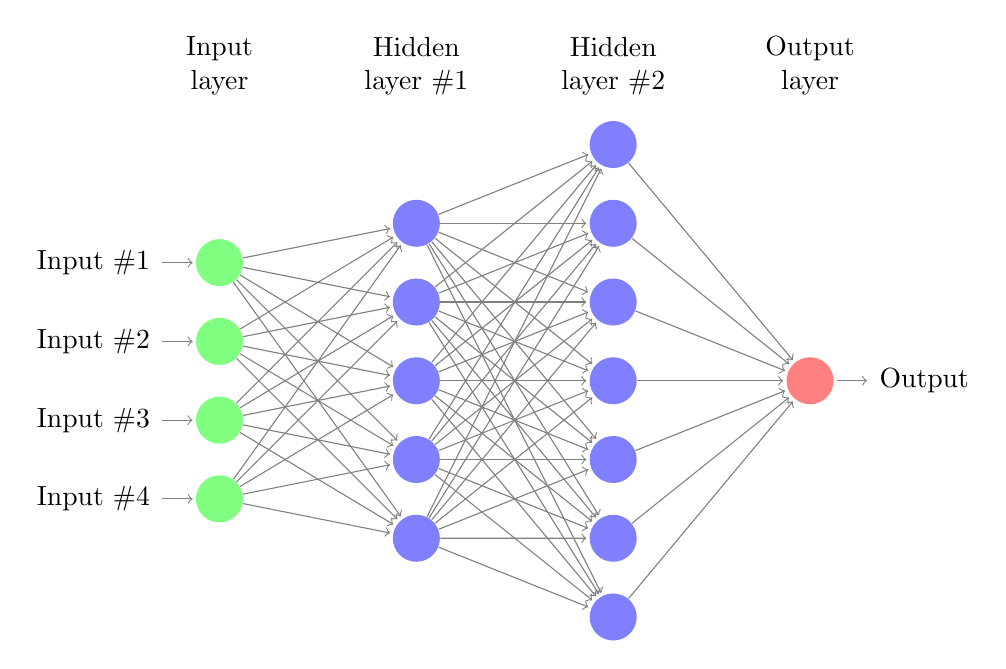
\begin{tikzpicture}[shorten >=1pt,->,draw=black!50, node distance=\layersep]
        \tikzstyle{every pin edge}=[<-,shorten <=1pt]
        \tikzstyle{neuron}=[circle,fill=black!25,minimum size=17pt,inner sep=0pt]
        \tikzstyle{input neuron}=[neuron, fill=green!50];
        \tikzstyle{output neuron}=[neuron, fill=red!50];
        \tikzstyle{hidden neuron}=[neuron, fill=blue!50];
        \tikzstyle{annot} = [text width=4em, text centered]
    
        % Draw the input layer nodes
        \foreach \name / \y in {1,...,4}
            \node[input neuron, pin=left:Input \#\y] (I-\name) at (0,-\y) {};
    
        % Draw the hidden layer 1 nodes
        \foreach \name / \y in {1,...,5}
            \path[yshift=0.5cm]
                node[hidden neuron] (H-\name) at (\layersep,-\y cm) {};
        
        % Draw the hidden layer 2 nodes
        \foreach \name / \y in {1,...,7}
            \path[yshift=1.5cm]
                node[hidden neuron] (G-\name) at (2*\layersep,-\y cm) {};
    
        % Draw the output layer node
        \node[output neuron,pin={[pin edge={->}]right:Output}, right of=G-4] (O) {};
    
        % Connect layers densely
        \foreach \source in {1,...,4}
            \foreach \dest in {1,...,5}
                \path (I-\source) edge (H-\dest);
        
        \foreach \source in {1,...,5}
            \foreach \dest in {1,...,7}
                \path (H-\source) edge (G-\dest);

        \foreach \source in {1,...,7}
            \path (G-\source) edge (O);
    
        % Annotate layers
        \node[annot,above of=G-1, node distance=1cm] (gl) {Hidden layer \#2};
        \node[annot,left of=gl] (hl) {Hidden layer \#1};
        \node[annot,left of=hl] {Input layer};
        \node[annot,right of=gl] {Output layer};
    \end{tikzpicture}
    \caption{\label{fig:neural-network}Architecture of a simple multilayer perceptron with an input layer, two hidden fully connected layers and an output layer.}
\end{figure}

\subsection*{Neural Networks}
Deep feedforward networks are models that let the information flow through forward to transform it into an output. This is the reason why they are called feedforward. They contain no feedback connections that would form a cyclic dependency. They are called networks because they represent several functions composed into an acyclic graph. Deep feedforward networks are also loosely inspired by neuroscience and that is where the word neural comes from. The term Neural Network (NN) stabilized as a different name for deep feedforward networks and it is used in the following sections and chapters.

Goal of Neural Network is to approximate some function $f^*$. In case of using a NN as a classifier, $y=f(\pmb x; \pmb \Theta)$ maps a vector input $\pmb x$ to a category $y$ while $\pmb \Theta$ are the parameters that result in a best approximation of $f^*$. Neural Networks consist of multiple layers connected into a chain and each of these layers can be represented by a function $f^{(i)}$ where $i$ is the index of layer. NN with 3 layers can be then mathematically expressed as $f(\pmb x)=f^{(3)}(f^{(2)}(f^{(1)}(\pmb x)))$.

Building blocks of layers are units. Each unit has a weight for each input, a bias and an activation function at the output. Example of a simple unit can be seen in \autoref{fig:nn-unit}. During the feedforward process, features of data are set as inputs and fed forward through the network. Every unit from the first hidden layer receives a value from each unit of input layer that it is connected to. It multiplies these values by their respective weights and adds them together. After that, the bias is added too. The result is then passed through the activation function and fed forward to units of the following layer. Activation functions often serve as some non-linear transformation. The feedforward computation for a single unit is then $h = g(\pmb w ^\top \pmb x + b)$, where $g$ is an activation function, $\pmb w$ is a vector of weights, $\pmb x$~is a vector of input values and $b$ is a bias. All vectors in formulas in this thesis are written in~bold.

\begin{figure}[!h]
    \centering
    \begin{tikzpicture}[
            node distance = 8mm and 20mm,
            start chain = going below,
            arro/.style = {-Latex},
            bloque/.style = {text width=4ex,
                inner sep=1pt,
                align=right,
                on chain
            },
        ]
        
        % inputs
        \node[bloque] (in-0) {\mbox{$+1$}};
        \foreach \i [count=\j] in {1, 2, 3}
            \node[bloque] (in-\j) {$x_{\i}$};
        % output
        \node (out) [circle, draw=black, minimum size=10mm, right=of $(in-1)!0.5!(in-2)$] {\Huge $\Sigma$};
        
        % conections
        \draw[arro] (in-0) -- (out) node[above, midway] {$b$};
        \foreach \i in {1,...,3}
            \draw[arro] (in-\i) -- (out) node[above, midway] {$w_{\i}$};
        
        % activation function
        \node (activation) [rectangle, draw=black, minimum size=6mm, right=of out] {\LARGE $\sigma$};
        \draw[arro] (out) -- (activation);
        
        % output
        \coordinate[right=of activation] (output);
        \draw[arro] (activation) -- (output) node[right] {$h$};
    \end{tikzpicture}
    \caption{\label{fig:nn-unit}Simple unit (also called neuron) of a layer of Neural Network. It has 3 inputs, bias and a sigmoid function as an activation function.}
\end{figure}

It is important to have a function that can evaluate how good the approximation of $f^*$ by $f$ is. This function is called loss or cost function and it measures the performance of NN by computing the error between the predicted values and expected values. Neural Networks often use a measure called Cross-Entropy which computes the difference between two probability distributions. Binary Cross-Entropy calculates the average number of bits required to represent an event from a distribution $Q$ by a distribution $P$, where $Q$ is the predicted distribution (approximated) and $P$ is the expected distribution (original) \cite{murphy2013machine}.

$$H(P, Q) = -\sum\limits_{x \in X} P(x) \log_2 Q(x) $$

The approximation of $f^*$ is called the training of the Neural Network. Parameters of NN that provide the best approximation cannot be calculated analytically, an optimization algorithm has to be used instead. Gradient descent is an example of iterative, gradient-based optimizer that is trying to minimize a loss function. Probably the most used optimization algorithm in Machine Learning, in general, is the Stochastic Gradient Descent (SGD). It~uses a small number of samples called a minibatch to compute the gradient and it applies it to improve the performance of the NN. Gradient itself is just the direction of the step towards an optimum, an important part of SGD is also the size of the step. This size is called a learning rate and it can be fixed during the training. For a loss function $L$, gradient descent requires computing:

$$ \nabla_{\pmb \Theta} J(\pmb \Theta) = \frac{1}{m} \sum\limits_{i=1}^{m} \nabla_{\pmb \Theta} L(f(\pmb {x}^{(i)}; \pmb \Theta), \pmb {y}^{(i)}) .$$

Improved versions of SGD are used as optimization algorithms. One of the disadvantages of SGD is the fixed learning rate and the difficulty of setting it correctly. It has a~significant impact on the training process. One way to improve the SGD is to use different learning rates for every parameter. Another way to improve it is by changing the learning rate throughout the training process. Both of these approaches are used in the Adam optimization algorithm that is used in this thesis. Adam algorithm uses the mean and uncentered variance of parameters to adapt the learning rates. It is computed as follows.

$$ \pmb s = \rho_1 \pmb s + (1 - \rho_1) \pmb g$$
$$ \pmb r = \rho_2 \pmb r + (1 - \rho_2) \pmb g \odot \pmb g$$
$$ \hat{\pmb s} = \frac{\pmb s}{1 - \rho_1} $$
$$ \hat{\pmb r} = \frac{\pmb r}{1 - \rho_2} $$
$$ \Delta \pmb \Theta = - \epsilon \frac{\hat{\pmb s}}{\sqrt{\hat{\pmb r}} + \delta} $$
$$ \pmb \Theta = \pmb \Theta + \Delta \pmb \Theta $$

\noindent Where:

$\pmb g$ is the computed gradient,

$\rho_1, \rho_2$ are exponential decay rates for moment estimates (mean and variance),

$\odot$ is an element-wise product,

$\pmb s$ is an updated biased first moment estimate,

$\pmb r$ is an updated biased second moment estimate,

$\hat{\pmb s}$ is a correct bias in the first moment,

$\hat{\pmb r}$ is a correct bias in the second moment,

$\epsilon$ is a step size and

$\delta$ is a small constant used for numerical stabilization.
\vspace{0.2cm}

The whole set of training data called a dataset is divided into minibatches to best suit an SGD-based optimization algorithm. The size of such minibatch can be from lower tens to higher hundreds. Minibatches should be randomly chosen from the dataset to prevent overfitting of the model. The optimization algorithm computes the gradient from the whole minibatch, then it computes the update of the parameters and applies it. Other options are to use a whole dataset as a training batch but that might result in a premature convergence and requires a lot of memory for large datasets. Another approach is to update the parameters for every single sample but that is computationally less efficient and it might be more difficult for the model to reach the optimum.

The computing of gradients is done by the backpropagation algorithm. The algorithm computes the gradient of the loss function with respect to the parameters of NN. The gradient is calculated as a derivative of a function and since layers of the networks are composed functions, the chain rule of calculus can be used. It states that:

$$\frac{\mathrm{d}x}{\mathrm{d}z} = \frac{\mathrm{d}x}{\mathrm{d}y}\frac{\mathrm{d}y}{\mathrm{d}z} .$$

\noindent Which can be generalized beyond the scalar case with partial derivatives. Suppose that $\pmb x \in \mathbb{R}^m$, $\pmb y \in \mathbb{R}^n$, $g: \mathbb{R}^m \rightarrow \mathbb{R}^n$, $f: \mathbb{R}^n \rightarrow \mathbb{R}$. If $\pmb y = g(\pmb x )$ and $z = f(\pmb y )$, then:

$$\frac{\partial z}{\partial x_i} = \sum\limits_{j} \frac{\partial z}{\partial y_j} \frac{\partial y_j}{\partial x_i} .$$

\newpage
\noindent Or, written in vector notation as:
    
$$ \nabla \pmb x ^z = \left( \frac{\partial \pmb y }{\partial \pmb x } \right) ^\top \nabla \pmb y ^z ,$$

\noindent where $\frac{\partial \pmb y }{\partial \pmb x }$ is the $n \times m$ Jacobian matrix of $\pmb g$. This is how the gradient is computed for every layer of NN with the backpropagation algorithm.

\subsection*{Convolutional Neural Networks}
Convolutional Neural Network (CNN) is a special kind of Neural Network that includes at least one layer that performs a mathematical operation called convolution instead of matrix multiplication. Specialization of these networks is data with grid-like topology, for example, time-series data that can be thought of as 1-dimensional grid or image data that are 2-dimensional grids of pixels. Such image data are used in this thesis as well.

In CNNs, convolution calculates a weighted sum, which means it takes a fixed number of values, multiples them with some constant and sums them together. This operation is done for the whole input. If the input is a 1-dimensional array, it starts at the beginning and computes the convolution for a fixed number of values. After that, it moves further in the 1-dimensional by some step and computes the convolution again. The result of this operation is the weighted sums arranged in a 1-dimensional array. \autoref{fig:1d-convolution} displays an~example of a~1-dimensional convolution.

\begin{figure}[!h]
    \centering
    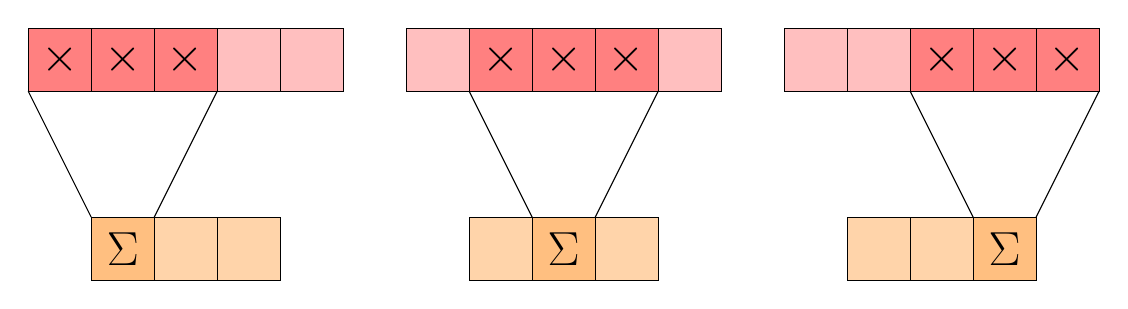
\begin{tikzpicture}[scale=0.8]
        \draw[fill={rgb:red,1;white,3}] (0, 3) rectangle (5, 4);
        \draw[fill={rgb:red,1;white,1}] (0, 3) rectangle (3, 4)  node[pos=0.5] {\LARGE $\times \  \times \  \times$};
        \draw (1, 3) -- (1, 4);
        \draw (2, 3) -- (2, 4);
        \draw (3, 3) -- (3, 4);
        \draw (4, 3) -- (4, 4);
        
        \draw (0, 3) -- (1, 1);
        \draw (3, 3) -- (2, 1);
        
        \draw[fill={rgb:orange,1;white,2}] (1, 0) rectangle (4, 1);
        \draw[fill={rgb:orange,1;white,1}] (1, 0) rectangle (2, 1) node[pos=0.5] {\LARGE $\Sigma$};
        \draw (2, 0) -- (2, 1);
        \draw (3, 0) -- (3, 1);
        
        \draw[fill={rgb:red,1;white,3}] (6, 3) rectangle (11, 4);
        \draw[fill={rgb:red,1;white,1}] (7, 3) rectangle (10, 4)  node[pos=0.5] {\LARGE $\times \  \times \  \times$};
        \draw (7, 3) -- (7, 4);
        \draw (8, 3) -- (8, 4);
        \draw (9, 3) -- (9, 4);
        \draw (10, 3) -- (10, 4);
        
        \draw (7, 3) -- (8, 1);
        \draw (10, 3) -- (9, 1);
        
        \draw[fill={rgb:orange,1;white,2}] (7, 0) rectangle (10, 1);
        \draw[fill={rgb:orange,1;white,1}] (8, 0) rectangle (9, 1) node[pos=0.5] {\LARGE $\Sigma$};
        \draw (8, 0) -- (8, 1);
        \draw (9, 0) -- (9, 1);
        
        \draw[fill={rgb:red,1;white,3}] (12, 3) rectangle (17, 4);
        \draw[fill={rgb:red,1;white,1}] (14, 3) rectangle (17, 4)  node[pos=0.5] {\LARGE $\times \  \times \  \times$};
        \draw (13, 3) -- (13, 4);
        \draw (14, 3) -- (14, 4);
        \draw (15, 3) -- (15, 4);
        \draw (16, 3) -- (16, 4);
        
        \draw (14, 3) -- (15, 1);
        \draw (17, 3) -- (16, 1);
        
        \draw[fill={rgb:orange,1;white,2}] (13, 0) rectangle (16, 1);
        \draw[fill={rgb:orange,1;white,1}] (15, 0) rectangle (16, 1) node[pos=0.5] {\LARGE $\Sigma$};
        \draw (14, 0) -- (14, 1);
        \draw (15, 0) -- (15, 1);
    \end{tikzpicture}
    \caption{\label{fig:1d-convolution}Example of 1-dimensional convolution with input size 5, kernel size 3 and step size 1.}
\end{figure}

The input of the convolution can be multidimensional. Weights used for the weighted sum are then arranged in a multidimensional array which is called a kernel. The output of the convolution is referred to as a feature map and it is multidimensional as well. The operation of convolution is often denoted with an asterisk. For a 2-dimensional case with image $I$ of size $m \times n$ and kernel $K$, the convolution is calculated as:

$$ S(i, j) = (I * K)(i, j) = \sum\limits_m \sum\limits_n I(m, n) K(i-m, j-n) .$$

Convolutional layers in comparison to normal layers in NN do not use matrix multiplication with weights that are trained. They perform convolution and instead of training weights, the neural network is trying to improve kernels to produce better results. Feature maps are then produced as an output.

The convolutional layer can be also used to perform downsampling. This can be achieved by setting the stride size to more than 1. The layer produces fewer values for the same input, approximately half of the values for stride size 2, third for stride of 3, and so on. Downsampling is often accompanied by an increasing number of kernels applied in one layer. Each convolution performs a different filtering operation, therefore, kernels are referred to as filters. For an example of image processing, the image's resolution is lower but the number of channels it is represented with is higher. Channels of the image are in this example the feature maps produced by the convolutional layer.

An important part of the convolutional layer is how it deals with the edges of input. When the input is not padded, the feature map on the output will have a different size than the input (as can be seen in \autoref{fig:1d-convolution}) but it uses only valid values. Therefore, this option is often referred to as \texttt{valid}. To keep the size the same, input has to be padded with zeros (as can be seen in \autoref{fig:2d-convolution}). This option of padding is called \texttt{same}.

\begin{figure}[!h]
    \centering
    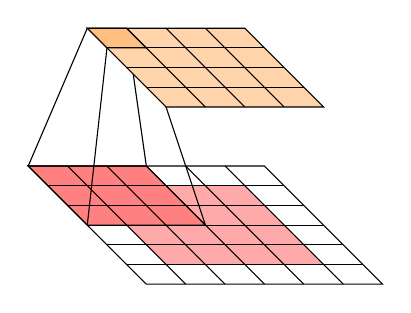
\begin{tikzpicture}[scale=1]
        \fill[fill={rgb:red,1;white,2}] (1, 0) -- (3, 0) -- (2, 1) -- (0, 1) -- cycle;
        \draw[fill={rgb:red,1;white,1}] (0, 0.5) -- (1.5, 0.5) -- (0.75, 1.25) -- (-0.75, 1.25) -- cycle;
        \draw (0.75, -0.25) -- (3.75, -0.25) -- (2.25, 1.25) -- (-0.75, 1.25) -- cycle;
        \draw (0.5, 0) -- (3.5, 0);
        \draw (0.25, 0.25) -- (3.25, 0.25);
        \draw (0, 0.5) -- (3, 0.5);
        \draw (-0.25, 0.75) -- (2.75, 0.75);
        \draw (-0.5, 1) -- (2.5, 1);
        \draw (1.25, -0.25) -- (-0.25, 1.25);
        \draw (1.75, -0.25) -- (0.25, 1.25);
        \draw (2.25, -0.25) -- (0.75, 1.25);
        \draw (2.75, -0.25) -- (1.25, 1.25);
        \draw (3.25, -0.25) -- (1.75, 1.25);
        
        \draw (0, 0.5) -- (0.25, 2.75);
        \draw (1.5, 0.5) -- (0.75, 2.75);
        \draw (0.75, 1.25) -- (0.5, 3);
        \draw (-0.75, 1.25) -- (0, 3);
        
        \draw[fill={rgb:orange,1;white,2}] (1, 2) -- (3, 2) -- (2, 3) -- (0, 3) -- cycle;
        \draw[fill={rgb:orange,1;white,1}] (0.25, 2.75) -- (0.75, 2.75) -- (0.5, 3) -- (0, 3) -- cycle;
        \draw (0.25, 2.75) -- (2.25, 2.75);
        \draw (0.5, 2.5) -- (2.5, 2.5);
        \draw (0.75, 2.25) -- (2.75, 2.25);
        \draw (0.5, 3) -- (1.5, 2);
        \draw (1, 3) -- (2, 2);
        \draw (1.5, 3) -- (2.5, 2);
    \end{tikzpicture}
    \caption{\label{fig:2d-convolution}Example of 2-dimensional convolution with input size 4, kernel size 3, step size~1, and padding size 1. Feature map has the same size as input because of the padding.}
\end{figure}

The main advantage of CNN is that it can capture the context of pixel values, it does not only process independent values without any connection between them. Another big advantage is its low memory requirements in comparison to how advanced results it produces. In normal NN, weight is only applied to a single value and then never used again in the feedforward process. But the CNN uses weights in a kernel multiple times when applying it to different values of the layer input, for example to pixels of an image. This reduces the number of parameters needed for training while not affecting the runtime. Another important advantage is equivariance. When explained on an example for image processing, it means that when the convolutional layer detects edge in some part of an image, the same detection can be done in other parts of the image and both results will be the same.

\section{\label{sec:generative-adversarial-networks}Generative Adversarial Networks}
Generative Adversarial Network (GAN) is a deep generative model. Its main goal is not classifying samples, as it was with previously mentioned models, but generating new samples. It is constructed from 2 specific models, one is used for generating new samples, therefore, it is called a generator.
The other one is called discriminator and its task is evaluating the probability of the provided sample not being generated from the generator. Architecture of a GAN can be seen in \autoref{fig:gan-architecture}. This creates a scenario where the two models are competing against each other and improving while doing so. The generator is trying to produce samples that are as close to real data as possible, so the discriminator cannot distinguish them.

\begin{figure}[!h]
    \centering
    \begin{tikzpicture}
        \draw (0, 3.5) rectangle (2.5, 4.5) node[pos=0.5, align=center] {Dataset};
        \draw [-{Latex[length=2.5mm]}] (2.5, 4) -- (6, 4);
        \draw (6, 3.25) rectangle (8, 4.75) node[pos=0.5, align=center] {Real\\sample};
        
        \draw [-{Latex[length=2.5mm]}] (8, 4) -- (9, 2.5);
        \draw [-{Latex[length=2.5mm]}] (8, 1) -- (9, 2.5);
        \draw[fill={rgb:red,1;white,3}] (9, 1.5) rectangle (11.5, 3.5) node[pos=0.5, align=center] {Discriminator};
        \draw [-{Latex[length=2.5mm]}] (11.5, 2.5) -- (12, 2.5);
        \draw (12, 1.75) rectangle (14.5, 3.25) node[pos=0.5, align=center] {Probability\\of being real};
        
        \draw (0, 0.5) rectangle (2.5, 1.5) node[pos=0.5, align=center] {Random noise};
        \draw [-{Latex[length=2.5mm]}] (2.5, 1) -- (3, 1);
        \draw[fill={rgb:cyan,1;white,3}] (3, 0) rectangle (5.5, 2) node[pos=0.5, align=center] {Generator};
        \draw [-{Latex[length=2.5mm]}] (5.5, 1) -- (6, 1);
        \draw (6, 0.25) rectangle (8, 1.75) node[pos=0.5, align=center] {Generated\\sample};
    \end{tikzpicture}
    \caption{\label{fig:gan-architecture}The architecture of Generative Adversarial Network where the generator produces images and the discriminator classifies them.}
\end{figure}

In this thesis, both of the models that are representing GAN are Neural Networks. There are multiple reasons to use those. As it is mentioned in \autoref{sec:deep-learning}, Neural Networks perform very well when it comes to samples whose features cannot be easily described. The feedforward process allows for a simple generating process and the backpropagation algorithm lets the network trained very efficiently. GANs in this thesis are using random noise as input for the generator. The goal of the generator is then to learn how to map the latent space from which the random noise comes to real data.

The generator can be described as function $G(\pmb z; \pmb \Theta_G)$, where $\pmb z$ is the random noise on the input and $\pmb \Theta_G$ are parameters of the NN. The output of the generator is sample $\pmb x$. The discriminator is represented by function $D(\pmb x; \pmb \Theta_D)$, where $\pmb x$ is a sample on the input and $\pmb \Theta_D$ are parameters of the NN \cite{NIPS2014_5423}. The output of the discriminator is a single scalar, probability of the sample being real and not generated by the generator. The discriminator is trained to assign a correct label to both real and generated samples, that means maximizing of $\log D(\pmb x)$. The generator is simultaneously trained to minimize $\log (1 - D(G(\pmb z))$. The training can be described as two-player minimax game with value function $V(D, G)$, where $\mathbb{E}_{x \sim P} [f(x)]$ is the expectation of $f(x)$ with respect to $P(x)$.

$$ \min\limits_G \max\limits_D V(D, G) =
\mathbb{E}_{\pmb x \sim p_{data} (\pmb x)}[\log D(\pmb x)] +
\mathbb{E}_{\pmb z \sim p_{z} (\pmb z)}[\log (1 - D(G(\pmb z))]$$

It is very important to carefully select the architecture of both models and their hyperparameters, otherwise the training of GAN can be unstable. It is essential to use dropout in the network architectures. Units should be stochastically dropped while computing the gradient for the generator to produce good results. GANs do not memorize the training dataset, they produce samples that were not part of the dataset neither they were close to training samples \cite{NIPS2014_5423}.

One option to train a GAN is described in this paragraph. The procedure can be divided into two parts, training of discriminator and training of generator. The discriminator is trained individually on a batch of samples, half of the batch is real training samples and the other half is generated samples. Samples are labeled to distinguish real from generated ones. The generator is trained in the whole GAN model but the discriminator's weights are not updated during this part of the training. On the input of the generator is a batch of random values. Samples are generated from the random values in the batch and evaluated by the discriminator. Error then backpropagates through the discriminator and updates the weights of the generator.

\subsection*{Generative Adversarial Networks for generating images}
Generating of image data is a task that can be very useful in real-life applications, therefore, it is a field worth exploring with Generative Adversarial Networks. Convolutional Neural Networks are used in most of the image classifying tasks and they produce good results when used in GANs too. A specific approach for designing of discriminator and generator model was used in this thesis and it is described in the following paragraphs.

Discriminator consists of multiple 2-dimensional convolutional layers that always reduce the resolution of the image to half while increasing the number of channels image is represented with. The generator is a mirrored version of the discriminator. It uses 2-dimensional transpose convolutional layers that double the resolution of an image while lowering the number of channels, as is shown in \autoref{fig:generator-architecture}. This architecture of both networks ensures that main features are learned as well as features representing small details \cite{karras2017progressive}.

\begin{figure}[!h]
    \centering
    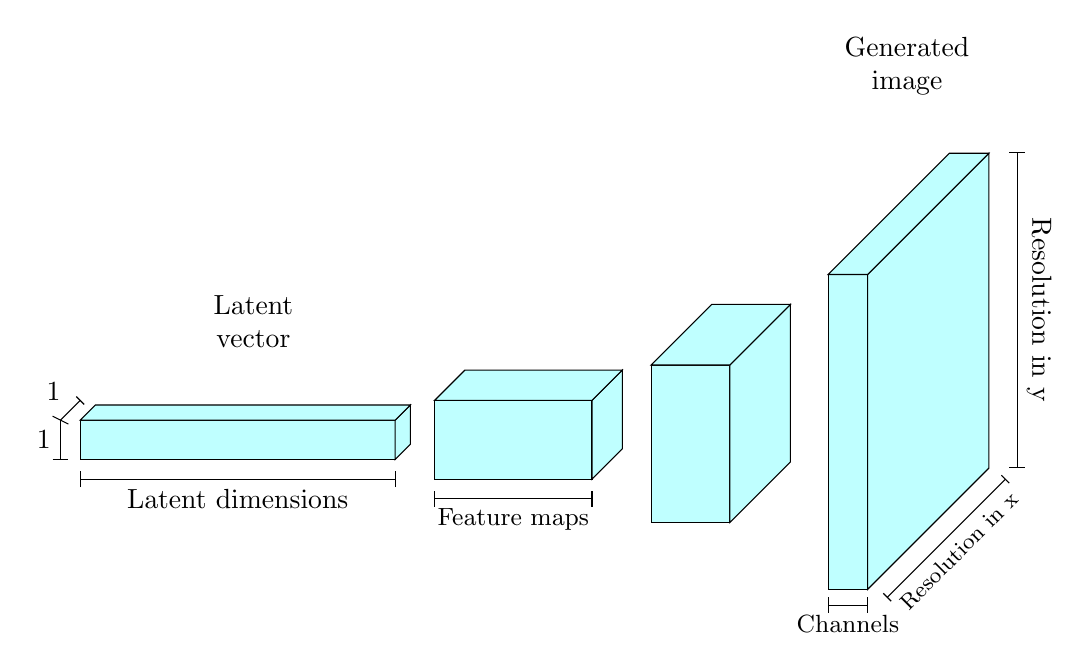
\begin{tikzpicture}
        \draw (-1.8, 1.25) node[align=center] {Latent\\vector};
        \draw (6.5, 4.5) node[align=center] {Generated\\image};
    
        \pgfmathsetmacro{\cubex}{4}
        \pgfmathsetmacro{\cubey}{0.5}
        \pgfmathsetmacro{\cubez}{0.5}
        \draw[black,fill={rgb:cyan,1;white,3}] (0,0,0) -- ++(-\cubex,0,0) -- ++(0,-\cubey,0) -- ++(\cubex,0,0) -- cycle;
        \draw[black,fill={rgb:cyan,1;white,3}] (0,0,0) -- ++(0,0,-\cubez) -- ++(0,-\cubey,0) -- ++(0,0,\cubez) -- cycle;
        \draw[black,fill={rgb:cyan,1;white,3}] (0,0,0) -- ++(-\cubex,0,0) -- ++(0,0,-\cubez) -- ++(\cubex,0,0) -- cycle;
        
        \draw (-4, -0.75) -- (0, -0.75) node[below, midway] {Latent dimensions};
        \draw (-4, -0.85) -- (-4, -0.65);
        \draw (0, -0.85) -- (0, -0.65);
        \draw (-4.25, -0.5) -- (-4.25, 0) node[left, midway] {1};
        \draw (-4.35, -0.5) -- (-4.15, -0.5);
        \draw (-4.35, 0.05) -- (-4.15, -0.05);
        \draw (-4.25, 0) -- (-4, 0.25) node[above left, midway] {1};
        \draw (-4.05, 0.30) -- (-3.95, 0.20);
        
        \pgfmathsetmacro{\cubex}{2}
        \pgfmathsetmacro{\cubey}{1}
        \pgfmathsetmacro{\cubez}{1}
        \draw[black,fill={rgb:cyan,1;white,3}] (2.5, 0.25, 0) -- ++(-\cubex,0,0) -- ++(0,-\cubey,0) -- ++(\cubex,0,0) -- cycle;
        \draw[black,fill={rgb:cyan,1;white,3}] (2.5, 0.25, 0) -- ++(0,0,-\cubez) -- ++(0,-\cubey,0) -- ++(0,0,\cubez) -- cycle;
        \draw[black,fill={rgb:cyan,1;white,3}] (2.5, 0.25, 0) -- ++(-\cubex,0,0) -- ++(0,0,-\cubez) -- ++(\cubex,0,0) -- cycle;
        
        \draw (0.5, -1) -- (2.5, -1) node[below, midway] {\small Feature maps};
        \draw (0.5, -1.1) -- (0.5, -0.9);
        \draw (2.5, -1.1) -- (2.5, -0.9);
        
        \pgfmathsetmacro{\cubex}{1}
        \pgfmathsetmacro{\cubey}{2}
        \pgfmathsetmacro{\cubez}{2}
        \draw[black,fill={rgb:cyan,1;white,3}] (4.25, 0.7, 0) -- ++(-\cubex,0,0) -- ++(0,-\cubey,0) -- ++(\cubex,0,0) -- cycle;
        \draw[black,fill={rgb:cyan,1;white,3}] (4.25, 0.7, 0) -- ++(0,0,-\cubez) -- ++(0,-\cubey,0) -- ++(0,0,\cubez) -- cycle;
        \draw[black,fill={rgb:cyan,1;white,3}] (4.25, 0.7, 0) -- ++(-\cubex,0,0) -- ++(0,0,-\cubez) -- ++(\cubex,0,0) -- cycle;
        
        \pgfmathsetmacro{\cubex}{0.5}
        \pgfmathsetmacro{\cubey}{4}
        \pgfmathsetmacro{\cubez}{4}
        \draw[black,fill={rgb:cyan,1;white,3}] (6, 1.85, 0) -- ++(-\cubex,0,0) -- ++(0,-\cubey,0) -- ++(\cubex,0,0) -- cycle;
        \draw[black,fill={rgb:cyan,1;white,3}] (6, 1.85, 0) -- ++(0,0,-\cubez) -- ++(0,-\cubey,0) -- ++(0,0,\cubez) -- cycle;
        \draw[black,fill={rgb:cyan,1;white,3}] (6, 1.85, 0) -- ++(-\cubex,0,0) -- ++(0,0,-\cubez) -- ++(\cubex,0,0) -- cycle;
        
        \draw (5.5, -2.35) -- (6, -2.35) node[below, midway] {\small Channels};
        \draw (5.5, -2.25) -- (5.5, -2.45);
        \draw (6, -2.25) -- (6, -2.45);
        \path (7.9, 3.4) edge node[sloped, anchor=center, above] {Resolution in y} (7.9, -0.6);
        \draw (7.8, 3.4) -- (8, 3.4);
        \draw (7.8, -0.6) -- (8, -0.6);
        \path (6.25, -2.25) edge node[sloped, anchor=center, below] {\footnotesize Resolution in x} (7.75, -0.75);
        \draw (6.2, -2.2) -- (6.3, -2.3);
        \draw (7.7, -0.7) -- (7.8, -0.8);
        
    \end{tikzpicture}
    \caption{\label{fig:generator-architecture}Feedforward process with data in generator with transpose convolution that gradually increases the image's resolution while lowering the number of image's representations.}
\end{figure}

Transpose convolution is computed almost the same way as a normal convolution. The difference is that it first adds a zero padding to the image \cite{dumoulin2016guide}. In case of doubling the resolution by using the stride size 2, zeros are added to the edges as well as between all the pixels. Edges may not be padded evenly if an image of exactly twice as high resolution should be produced. Then a normal convolution with stride 1 and given kernel is performed and a feature map with higher resolution is produced. \autoref{fig:transposed-convolution} provides an example of a~transposed convolution.

\begin{figure}[!h]
    \centering
    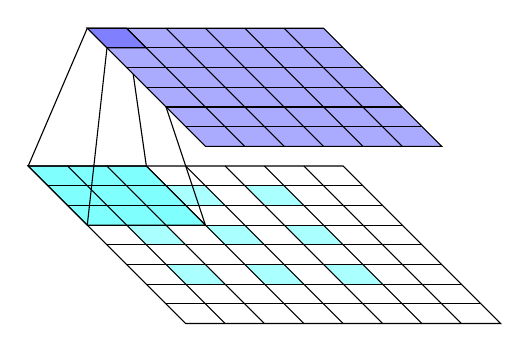
\begin{tikzpicture}[scale=1]
        \fill[fill={rgb:cyan,1;white,2}] (0.25, 0.75) -- (0.75, 0.75) -- (0.5, 1) -- (0, 1) -- cycle;
        \fill[fill={rgb:cyan,1;white,2}] (1.25, 0.75) -- (1.75, 0.75) -- (1.5, 1) -- (1, 1) -- cycle;
        \fill[fill={rgb:cyan,1;white,2}] (2.25, 0.75) -- (2.75, 0.75) -- (2.5, 1) -- (2, 1) -- cycle;
        \fill[fill={rgb:cyan,1;white,2}] (0.75, 0.25) -- (1.25, 0.25) -- (1, 0.5) -- (0.5, 0.5) -- cycle;
        \fill[fill={rgb:cyan,1;white,2}] (1.75, 0.25) -- (2.25, 0.25) -- (2, 0.5) -- (1.5, 0.5) -- cycle;
        \fill[fill={rgb:cyan,1;white,2}] (2.75, 0.25) -- (3.25, 0.25) -- (3, 0.5) -- (2.5, 0.5) -- cycle;
        \fill[fill={rgb:cyan,1;white,2}] (1.25, -0.25) -- (1.75, -0.25) -- (1.5, 0) -- (1, 0) -- cycle;
        \fill[fill={rgb:cyan,1;white,2}] (2.25, -0.25) -- (2.75, -0.25) -- (2.5, 0) -- (2, 0) -- cycle;
        \fill[fill={rgb:cyan,1;white,2}] (3.25, -0.25) -- (3.75, -0.25) -- (3.5, 0) -- (3, 0) -- cycle;
        \draw[fill={rgb:cyan,1;white,1}] (0, 0.5) -- (1.5, 0.5) -- (0.75, 1.25) -- (-0.75, 1.25) -- cycle;
        \draw (1.25, -0.75) -- (5.25, -0.75) -- (3.25, 1.25) -- (-0.75, 1.25) -- cycle;
        % horizontal lines from top to down
        \draw (-0.5, 1) -- (3.5, 1);
        \draw (-0.25, 0.75) -- (3.75, 0.75);
        \draw (0, 0.5) -- (4, 0.5);
        \draw (0.25, 0.25) -- (4.25, 0.25);
        \draw (0.5, 0) -- (4.5, 0);
        \draw (0.75, -0.25) -- (4.75, -0.25);
        \draw (1, -0.5) -- (5, -0.5);
        % vertical lines from left to right
        \draw (-0.25, 1.25) -- (1.75, -0.75);
        \draw (0.25, 1.25) -- (2.25, -0.75);
        \draw (0.75, 1.25) -- (2.75, -0.75);
        \draw (1.25, 1.25) -- (3.25, -0.75);
        \draw (1.75, 1.25) -- (3.75, -0.75);
        \draw (2.25, 1.25) -- (4.25, -0.75);
        \draw (2.75, 1.25) -- (4.75, -0.75);
        
        \draw (0, 0.5) -- (0.25, 2.75);
        \draw (1.5, 0.5) -- (0.75, 2.75);
        \draw (0.75, 1.25) -- (0.5, 3);
        \draw (-0.75, 1.25) -- (0, 3);
        
        \draw[fill={rgb:blue,1;white,2}] (1.5, 1.5) -- (4.5, 1.5) -- (3, 3) -- (0, 3) -- cycle;
        \draw[fill={rgb:blue,1;white,1}] (0.25, 2.75) -- (0.75, 2.75) -- (0.5, 3) -- (0, 3) -- cycle;
        % horizontal lines from top to down
        \draw (0.25, 2.75) -- (3.25, 2.75);
        \draw (0.5, 2.5) -- (3.5, 2.5);
        \draw (0.75, 2.25) -- (3.75, 2.25);
        \draw (1, 2) -- (4, 2);
        \draw (1.25, 1.75) -- (4.25, 1.75);
        % vertical lines from left to right
        \draw (0.5, 3) -- (2, 1.5);
        \draw (1, 3) -- (2.5, 1.5);
        \draw (1.5, 3) -- (3, 1.5);
        \draw (2, 3) -- (3.5, 1.5);
        \draw (2.5, 3) -- (4, 1.5);
    \end{tikzpicture}
    \caption{\label{fig:transposed-convolution}Transposed convolution used to double the size of image input. Input of size~3 is padded with zeros on the edges as well as between the pixels. The edges have to be padded unevenly. Input is then convolved with a kernel of size 3 with stride size 1, and the size of the feature map will be 6. Notice that the stride size of this convolution is 1 but in the settings of the transposed convolution would be the stride size 2.}
\end{figure}


\section{\label{sec:image-databases}Image databases}
Image classification is an often implemented task in practice but also for educational purposes. For that reason, there are many databases of labeled images available online for anyone to use. Generative Adversarial Networks can be trained on any images and do not even require the images to be labeled. The only requirement is an equal resolution of all images and preferably also some common features between all images. A database can contain photographs of animals, or photographs of vehicles for example, but not both of these categories.

\subsection*{\label{sec:mnist-database}Handwritten digits}
Modified National Institute of Standards and Technology (MNIST) database is one of the most commonly used databases for educational purposes in image processing \cite{lecun-mnisthandwrittendigit-2010}. It contains images of handwritten digits from 0 to 9 that are scaled and cropped to have a similar size and be positioned in the middle of the image as can be seen in \autoref{fig:mnist-examples-different}. No preprocessing of images has to be done beforehand. Images have a resolution of $28 \times 28$ pixels and are grayscale, which means only one value represents every pixel. In most cases, this value is an unsigned integer in the range between 0 and 255. Each image is labeled with the value of its digits, which gives 10 classes in total. The whole database contains 70000 samples from which 60000 are meant for training and 10000 for testing of the trained model.

\begin{figure}[!h]
    \centering
    
\includegraphics[scale=3]{figures/mnist/example_6_4337.png}
    
\includegraphics[scale=3]{figures/mnist/example_0_10705.png}
    
\includegraphics[scale=3]{figures/mnist/example_4_10104.png}
    
\includegraphics[scale=3]{figures/mnist/example_3_10074.png}
    \caption{\label{fig:mnist-examples-different}Examples of different digits from the MNIST digit database.}
\end{figure}

MNIST database is an ideal choice when starting the implementation of image processing neural network. Low resolution and only one channel of each image make the task as~easy as possible. The training time is short and the neural network can be constructed from a relatively small number of layers (under ten). Therefore, it is not necessary to use a lot of computational power. Another advantage is the small size of images, they can be loaded into memory and used at the same time without reloading. Images of the same digit can be different because they are all handwritten. This is shown in \autoref{fig:mnist-examples-same}. Such variety presents a difficult enough challenge for the neural network.

\begin{figure}[!h]
    \centering
    
\includegraphics[scale=3]{figures/mnist/example_1_55832.png}
    
\includegraphics[scale=3]{figures/mnist/example_1_10364.png}
    
\includegraphics[scale=3]{figures/mnist/example_1_10048.png}
    
\includegraphics[scale=3]{figures/mnist/example_1_55870.png}
    \caption{\label{fig:mnist-examples-same}Examples of identical digits from the MNIST digit database. Even the same digits can be written in different ways.}
\end{figure}

\newpage
\subsection*{\label{sec:lfw-database}Labeled Faces in the Wild}
Labeled Faces in the Wild (LFW) is a public database of color images of faces collected from the web \cite{LFWTech}. The database contains 13233 photos of 5749 people with 1680 out of them on two or more photos. Each image is labeled with the name of the person on it. The resolution of original images is $250 \times 250$ pixels and each pixel is represented by 3 channels (red, green, and blue). Examples from the LFW database can be seen in \autoref{fig:lfw-original}.

\begin{figure}[!h]
    \centering
    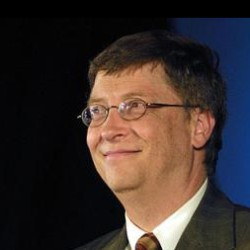
\includegraphics[scale=0.4]{figures/lfw/original_Bill_Gates_0002.jpg}
    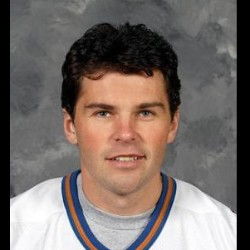
\includegraphics[scale=0.4]{figures/lfw/original_Jaromir_Jagr_0001.jpg}
    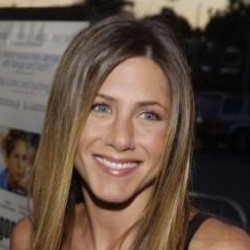
\includegraphics[scale=0.4]{figures/lfw/original_Jennifer_Aniston_0015.jpg}
    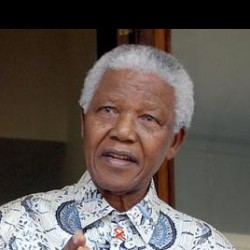
\includegraphics[scale=0.4]{figures/lfw/original_Nelson_Mandela_0004.jpg}
    \caption{\label{fig:lfw-original}Examples from LFW database.}
\end{figure}

Faces are located in the center of the picture and can point also partially sideways, not only to the front. Peoples' faces can be covered with headwear or glasses. As the database's name suggests, images have a large variety of backgrounds behind the photographed people. All of these properties make the task of image processing more challenging but also closer to real-life problems.

LFW database is good for research and education but should not be used for commercial purposes. The reason is not so high variability of the people in the images. There are very few children, no babies, almost no people over 80 years old, and a relatively small amount of women. Also, many ethnicities are represented in a small portion or not at all. The size of the database is also not big enough for strong statistical conclusions about subgroups.

Faces from the LFW database can be used as a next step in developing an image processing neural network. However, they should not be used as a training database for the finalized network because of the reasons mentioned.

\subsection*{\label{sec:ffhq-database}Flickr-Faces-HQ}
Flickr-Faces-HQ (FFHQ) is a database of high-quality images of faces created as~a~benchmark for Generative Adversarial Networks \cite{karras2018stylebased}. Images were extracted from photographs uploaded to service Flickr and then aligned, cropped and saved as \texttt{png} files. Only images with licenses for free use for non-commercial purposes were used for this database. The size of the database is 70000 images with a resolution of $1024 \times 1024$ pixels. Creators of this database offer also thumbnails of each image with a resolution of $128 \times 128$ pixels and original images from which the faces where extracted.

FFHQ database contains photographs of people with a wide variety of ages, ethnicity, and image background. Also, people wearing different kinds of headwear and glasses are included as shown in \autoref{fig:ffhq-examples}. Faces are photographed from different angles and in~different light conditions. These properties make the database ideal for the training of image processing neural networks.

\begin{figure}[!h]
    \centering
    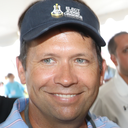
\includegraphics[scale=0.8]{figures/ffhq/example1_00011.png}
    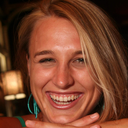
\includegraphics[scale=0.8]{figures/ffhq/example2_00001.png}
    
\includegraphics[scale=0.8]{figures/ffhq/example3_00005.png}
    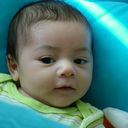
\includegraphics[scale=0.8]{figures/ffhq/example4_00000.png}
    \caption{\label{fig:ffhq-examples}Examples from FFHQ database.}
\end{figure}

\subsection*{Other databases of faces}
CelebFaces Attributes (CelebA) database contains 202599 photographs of celebrities \cite{liu2015faceattributes}. Each image has 40 binary attribute annotations, such as the person's facial expression and shape of the face, whether the person is wearing glasses, hat or other accessories, and other features of a face. It contains a large variety of poses and backgrounds of images.

There is also a large number of databases that have a wide variety of images sorted into classes. For the training of GANs, only one class can be used at a time. Some of these databases are described in the following paragraphs.

ImageNet is an image database that is organized into classes according to the WordNet\footnote{WordNet\textregistered is a large lexical database of English, more information at \url{https://wordnet.princeton.edu/}} hierarchy \cite{imagenet_cvpr09}. It contains about 14 million images from 100000 classes that are supposed to serve for research and educational purposes.

LSUN database contains around one million images of all kinds \cite{yu2015lsun}. They are labeled for each of 10 scene categories and 20 object categories. It uses a crowdsourcing platform for labeling the images and therefore can grow in size.

The CIFAR-10 and CIFAR-100 are databases with a large variety of images sorted into 10 and 100 classes respectively \cite{cifar}. They both contain 60000 color images with a resolution of $32 \times 32$ pixels. Images in this database are subsets of the 80 million tiny images database \cite{tinyimages}.

\chapter{\label{chap:implementation}Implementation of Generative Adversarial Network}
All the Generative Adversarial Networks (GANs) mentioned in this thesis are implemented in \texttt{Python 3} with \texttt{TensorFlow 2} library through \texttt{Keras} API, \texttt{NumPy} library for advanced mathematical operations, and other libraries for specific smaller tasks. \texttt{TensorFlow} is a~deep learning \texttt{Python} library and it provides users with an easy way to design, train, and evaluate neural networks. Very important is also an option to predict with the neural network, which is also the case for generating data with GAN. Using \texttt{Keras} API on top of the \texttt{TensorFlow} library makes the building of neural networks more intuitive.

The code for every GAN usually consists of several similar parts. Common properties of each part are described in \autoref{sec:common-gans}. In the following sections are mentioned differences for each specific one. The first implemented GAN in this thesis generates images of handwritten digits and it is described in \autoref{sec:mnist-gan}. In the next \autoref{sec:lfw-gan}, are explained the differences in implementation of a GAN for images of faces from the LFW database. Finally, \autoref{sec:ffhq-gan} informs about the details of implementing GAN for high-quality images of faces from the FFHQ database.

\section{\label{sec:common-gans}Common segments of every Generative Adversarial Network}
Training of every GAN has to start with the loading of the training data. In most cases, the data has to be also preprocessed in some way. Generator in GAN uses a random noise as an input, therefore, it is necessary to have a function that generates the random noise in a format that is accepted by the generator. The architecture of both discriminator and generator has also some common properties which are described in this section. They are always somehow connected into the whole GAN, in this thesis, it is done with another model. After the models are defined, they can be trained. It is necessary to monitor the training and evaluate the results to achieve the best possible generated images. When the training is finished, the generator can be used for generating new data.

\subsection*{\label{sec:common-loading}Loading of training images}
At first, images have to be loaded into memory and in many cases also preprocessed. The preparation of images can consist of changing the resolution and cropping the image that leads to the resolution being easily factorized to small prime numbers, which is very useful for GANs. The number of channels of an image can also be altered (for example converting a color image to grayscale). Training data, in this case, an image database, are usually referred to as a dataset.

Neural networks process inputs with weights with small values \cite{Goodfellow-et-al-2016}, therefore, it is a~good practice to represent channel of each pixel by a value between 0 and 1, otherwise the weights can increase to large numbers and make the network unstable and unable to generalize well. In many cases, conversion of input values must be done because of pixels being represented by unsigned integer values from 0 to 255.

\subsection*{Generating points in latent space}
Points from latent space are necessary for GANs because they are used as an input for the generator. The dimensionality of latent space can vary from lower tens to higher hundreds. A certain power of number 2 is usually used as the number of dimensions. This point stores all the information about the generated result. The generator from trained GAN is used as a tool that deterministically generates the result from this point.

In this thesis, the latent vectors correspond to a random point on an $n$-dimensional hypersphere, where $n$ is the dimensionality of the latent space. That means that squared values in all dimensions of one latent vector have to sum up to a chosen constant which is the hypersphere's radius squared. The radius of the hypersphere is set to 1 in this thesis. Muller's algorithm is used to produce uniform random values with this property \cite{marsaglia1972}. The random point on a hypersphere is computed with the following formulas, where $d$ is a dimension index, $n$ is the dimensionality of the latent space, and $Y_d$ is the computed coordinate in dimension $d$. 

$$ S = \sum\limits_{d=0}^n X_d^2, \quad \text{where} \quad X_d \sim \mathcal{N}(0, 1)$$
$$ Y_d = \frac{X_d}{\sqrt{S}} $$

\subsection*{Building the model of discriminator}
The discriminator is a sequential model, which means its layers are saved in a linear stack. Input is an image and output is a value between 0 and 1 representing the probability that the image is real.

Very important layers in the model are 2-dimensional convolutional layers (Conv2D). The operation of convolution applies a filter to an image to obtain its feature map. Each feature map stores some information about the image. Filter used for obtaining each of all feature maps is the trained parameter of the convolutional layer. After the first convolution image is no longer represented with channels of image's resolution but with feature maps. These feature maps are then handled in the following layers.

Convolutional layers in discriminator decrease image's (and feature maps') resolution to half by using the stride of 2 and \uv{same} padding. Kernel size can vary in different cases but the size of 3 is used in many cases \cite{karras2017progressive}. The number of filters is usually a power of 2 in the range between 32 and 512. The more convolutions are applied the higher number of filters is used. That way more feature maps are obtained to represent the image.

The convolutional layer is followed by a layer with a leaky version of a Rectified Linear Unit (LeakyReLU) as an activation function.

$$ f(x) =
    \begin{cases}
        x           & \quad \text{if } x \geq 0 \\
        \alpha x    & \quad \text{if } x < 0
    \end{cases}
$$

\noindent This function is easy to compute because it consists of two linear parts but it can still learn complex structures in data because of its nonlinearity. These two properties make LeakyReLU a good activation function for deep neural networks. The steepness of the function for $x < 0$ can be set. An example of LeakyReLU can be seen in \autoref{fig:leakyrelu}.

\begin{figure}[!h]
    \centering
    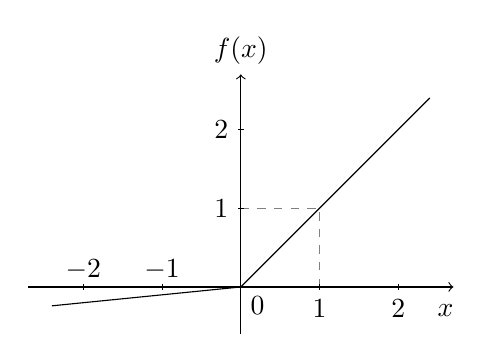
\begin{tikzpicture}
        \draw[->] (-2.7, 0) -- (2.7, 0);
        \draw (2.6, -0.3) node[] {$x$};
        \draw[->] (0, -0.6) -- (0, 2.7) node[above] {$f(x)$};
        \draw[very thin, dashed, color=gray] (1, 0) -- (1, 1);
        \draw[very thin, dashed, color=gray] (0, 1) -- (1, 1);
        \foreach \y/\ytext in {1, 2} 
            \draw (1pt, \y cm) -- (-1pt, \y cm) node[left] {$\ytext$};
        \foreach \x/\xtext in {1, 2} 
            \draw (\x cm,1pt) -- (\x cm,-1pt) node[below] {$\xtext$};
        \foreach \x/\xtext in {-2, -1} 
            \draw (\x cm,1pt) -- (\x cm,-1pt) node[above] {$\xtext$};
        \draw (0, 0) node[below right] {$0$};
        \draw[domain=0:2.4,smooth,variable=\x] plot ({\x},{\x});
        \draw[domain=-2.4:0,smooth,variable=\y] plot ({\y},{0.1*\y});
    \end{tikzpicture}
    \caption{\label{fig:leakyrelu}An example of Leaky Rectified Linear Unit.}
\end{figure}

After that is applied a layer that drops out a certain number of nodes. This layer is called Dropout and its drop out rate are set by a value between 0 and 1. It prevents the network from overfitting to the training samples.

The combination of the Conv2D layer, LeakyReLU activation function, and Dropout layer repeats multiple times. In the end, the image is transformed into a 1-dimensional list using the Flatten layer. This layer has no trainable weights, it is only used as a preparation for the following Dense layer. Dense means that it uses connections of all nodes between layers, in other words, it is fully connected. In this case, it connects all nodes from the Flatten layer to one node representing the probability of the input image being real. This value is normalized by the sigmoid activation function to values between 0 and 1. The shape of the sigmoid function is shown in \autoref{fig:sigmoid}.

$$ f(x) = \frac{1}{1 + e^{-x}} $$

\begin{figure}[!h]
    \centering
    \begin{tikzpicture}[yscale=2]
        \draw[->] (-3.7, 0) -- (3.7, 0);
        \draw (3.6, -0.15) node[] {$x$};
        \draw[->] (0, 0) -- (0, 1.4) node[above] {$f(x)$};
        \draw[very thin, dashed, color=gray] (-3.65, 1) -- (3.65, 1);
        \foreach \x/\xtext in {-3, -2, -1, 0, 1, 2, 3} 
            \draw (\x cm,1pt) -- (\x cm,-1pt) node[anchor=north] {$\xtext$};
        \draw (1pt,1 cm) -- (-1pt,1 cm);
        \draw (0, 1) node[above right] {$1$};
        \draw (2pt,0.5 cm) -- (-2pt,0.5 cm);
        \draw (0.4, 0.4) node[] {$\frac{1}{2}$};
        \draw[domain=-3.6:3.6,smooth,variable=\x] plot ({\x},{1/(1 + exp(-\x))});
    \end{tikzpicture}
    \caption{\label{fig:sigmoid}Sigmoid function.}
\end{figure}

The optimization algorithm used when training discriminator is Adam. This algorithm updates every weight with its own learning rate. Learning rates also adapt during the training by using the first and second moments of the gradient. Thanks to these advantages it is widely recommended to be used in Deep Neural Networks. For GANs in this thesis, the learning rate is set to $0.0002$ and exponential decay rate for the first moment (mean) estimates to $0.5$.

The loss function that is being minimized is the Cross-Entropy. Likelihood of image being real (belonging to class 1) or not (belonging to class 0) is a binary classification problem. Cross-Entropy is advised to be used for this type of problem.

\subsection*{Building the model of generator}
The generator is also a sequential model and in most cases, it consists of multiple transpose convolution layers that are used to increase the resolution of the image. It is basically a~mirrored version of the discriminator. Input is a point from latent space and output is a~generated image.

Generator first makes many low-resolution representations of the desired image. The dense layer can be used to connect the input array of random numbers with the low-resolution representations of that image. LeakyReLU is applied as the following layer to improve the generalization of the model. After that, it is necessary to reshape the array to three dimensions -- two for the image itself and one for all of the image representations. Reshape layers can be used for this purpose.

Two-dimensional transposed convolutional layers (Conv2DTranspose) are then applied to increase the resolution of the image. The transpose convolution is described in \autoref{sec:generative-adversarial-networks}. The input image can be thought of as a feature map and trained weights are actually filters of the transpose convolution. Doubling of resolution of an image is achieved by setting the stride to 2 and padding to \uv{same}. The more transpose convolutions are used, the fewer filters are usually used, which means the number of image's representations is lower. The Conv2DTranspose layer is often followed by a LeakyReLU layer for generalization improvement.

When the desired resolution of the image is obtained, one convolutional layer (Conv2D) can be used to convert all the representations of an image to channels (one channel for grayscale images or three channels for color images). The number of filters is the number of channels in the final image, the stride is set to 1 and padding to \uv{same} to keep the resolution of the image unchanged. The size of the kernel can vary in different situations. The sigmoid activation function is then applied to keep the pixel values between 0 and 1.

\subsection*{Connecting discriminator and generator together into one model}
Generative Adversarial Network itself is represented by a sequential model as well. It consists of discriminator and generator by themselves. The discriminator is not trained in this model, only the generator's weights are updated according to the discriminator's performance on generated images. That means that after discriminator evaluates the probability of provided images being real, backpropagation goes through the discriminator and then generator but only updates the weights in the generator. Training optimization is done with the Adam algorithm, the learning rate is set to $0.0002$ and exponential decay rate for the first moment (mean) estimates to $0.5$. Binary Cross-Entropy is used as a loss function.

\subsection*{Training of Generative Adversarial Network}
The training consists of a~certain number of epochs (hundreds or thousands). Epoch is an~iteration over the whole dataset of images. In each epoch, there is training done with images grouped into batches. The size of one batch can be in the lower hundreds. It is usually some power of two because these sizes can use hardware resources more efficiently~\cite{Goodfellow-et-al-2016}. The number of these batches used to train the GAN in one epoch is the number of available images for training divided by the size of the batch.

First comes the training of standalone discriminator. It is provided with a batch consisting of real and generated images and its task is to determine which one is real and which one is generated. This training of discriminator is done using the \texttt{train\_on\_batch} function from \texttt{Keras} API that updates the weights of the discriminator.

After that, the generator is trained in the whole GAN model. It provides the discriminator with a new batch of generated images. The discriminator determines whether the images are real or generated and then the backpropagation is used to update the generator weights. Once again, the \texttt{train\_on\_batch} function from \texttt{Keras} API is used for this task.

Both discriminator and generator are evaluated after each epoch. The discriminator is evaluated by recognizing real images, the generator is evaluated by discriminator's ability to recognize its generated images. Information about training loss of both models is printed after training on each batch.

\subsection*{Evaluation of results and monitoring of training}
There is no objective way to automatically evaluate generated images, the human eye has to decide about their quality. There is still the option of reviewing generated images with the discriminator but it depends on how good the discriminator is in recognizing real and generated images from each other. Discriminator can be tested the same way by providing it with real images and expecting to evaluate them all as real. This evaluation can be done with \texttt{evaluate} function from \texttt{Keras} API.

It is very important to monitor the process of training to know if the model is making progress. This can be done by following the scalar training loss that is returned by \texttt{train\_on\_batch} function from \texttt{Keras} API during the training. After a few epochs of training, these values should be balanced. If, for example, training loss of discriminator approaches 0 and training loss of generator increases above 10 and further, the model is probably not improving. Its design or training process should be changed to improve performance.

\subsection*{Generating new images from Generative Adversarial Network}
New images are generated from the trained generator model (not the whole GAN). For this reason, it is necessary to save the whole generator model or its weights after the training. If only weights are saved, the exact same generator model has to be defined before loading the weights and generating new images. When the model is loaded, it has to be provided with a point from latent space and then a new image can be generated with the \texttt{predict} function from \texttt{Keras} API.

\section{\label{sec:mnist-gan}Generating images of handwritten digits}
It is very useful to start implementing GAN for simpler images than photographs of faces. One of the very basic image databases is the Modified National Institute of Standard and Technology (MNIST) handwritten digit database. The resolution of these images is $28\times 28$ pixels. Every image is also labeled with the number that the handwritten digit represents. Further information about the MNIST database can be found in \autoref{sec:mnist-database}.

\subsection*{Loading and preparing images}
MNIST digit database can be obtained from the \texttt{TensorFlow} library via \texttt{Keras} API using the \texttt{load\_data} function. The dataset comes in two lists (train and test images) with shape (\textit{number of images}, 28, 28) together with the labels in two additional lists. There is no need for labels when training a GAN, the learning process is unsupervised. Only images for training are needed, testing and training is done simultaneously using newly generated images and the training images. Therefore the sets of 60000 training images and 10000 images can be merged into one and used.

Each pixel is represented with an unsigned integer value from 0 to 255. As mentioned in \autoref{sec:common-loading}, it is better practice to convert the values to floats and normalize them to range between 0 and 1. It is also necessary to update the number of dimensions to have the grayscale channel as an additional dimension. The shape of the training dataset is now (70000, 28, 28, 1) -- the grayscale value of each pixel is in its list.

The size of the digits from the MNIST database is $28\times 28$ pixels. Prime factors of number 28 are 2 and 7. And if the image is grown gradually, that means that at a certain point there has to a big step to make the image 7 times larger in pixel size. This big step is represented by many trainable weights in a layer of the generator. If a neural network has too many weights in one layer, the training can be time consuming and unstable.

To optimize this process, every image can be changed to a size of $32\times 32$ pixels by just adding 2 pixels with 0 values on each side. This will not affect any of the results because each digit image already has 0 values on the sides. Resizing of images just by adding zeros is a very fast process that will not affect the training speed almost at all. Number 32 has only one prime factor and that is number 2. Therefore the image can be grown from $4\times 4$ pixels up to $32\times 32$ pixels just by small steps of making it 2 times larger. The generator neural network will have more layers but it will be able to generate more precise images and the training will be faster. The shape of the final training dataset will be (70000, 32, 32, 1).

\subsection*{Architecture of Generative Adversarial Network}
This GAN uses latent space with 64 dimensions. The architecture of the discriminator model can be seen in \autoref{tab:gan-mnist-discriminator} and the generator model in \autoref{tab:gan-mnist-generator}.

\begin{table}
    \begin{center}
        \begin{tabular}{ |m{5em}|m{9em}|l|r| }
            \hline
                Layer & Settings & Shape & \multicolumn{1}{l|}{Parameters} \\ 
            \hline
            \hline
                Input & & (32, 32, 1) & 0 \\
            \hline
                Conv2D & \mbox{Filter count: 32} \mbox{Kernel size: (1, 1)} \mbox{Stride size: (1, 1)} & \multirow{3}{6em}{(32, 32, 32)} & 64 \\
            \cline{1-2} \cline{4-4}
                LeakyReLU & Alpha: 0.2 & & 0 \\
            \cline{1-2} \cline{4-4}
                Dropout & Rate: 0.4 & & 0 \\
            \hline
                Conv2D & \mbox{Filter count: 32} \mbox{Kernel size: (3, 3)} \mbox{Stride size: (2, 2)} & \multirow{3}{6em}{(16, 16, 32)} & 9~248 \\
            \cline{1-2} \cline{4-4}
                LeakyReLU & Alpha: 0.2 & & 0 \\
            \cline{1-2} \cline{4-4}
                Dropout & Rate: 0.4 & & 0 \\
            \hline
                Conv2D & \mbox{Filter count: 64} \mbox{Kernel size: (3, 3)} \mbox{Stride size: (2, 2)} & \multirow{3}{6em}{(8, 8, 64)} & 18~496 \\
            \cline{1-2} \cline{4-4}
                LeakyReLU & Alpha: 0.2 & & 0 \\
            \cline{1-2} \cline{4-4}
                Dropout & Rate: 0.4 & & 0 \\
            \hline
                Conv2D & \mbox{Filter count: 64} \mbox{Kernel size: (3, 3)} \mbox{Stride size: (2, 2)} & \multirow{3}{6em}{(4, 4, 64)} & 36~928 \\
            \cline{1-2} \cline{4-4}
                LeakyReLU & Alpha: 0.2 & & 0 \\
            \cline{1-2} \cline{4-4}
                Dropout & Rate: 0.4 & & 0 \\
            \hline
                Flatten & & (1024) & 0 \\
            \hline
                Dense & \mbox{Units: 1} \mbox{Activation: Sigmoid} & (1) & 1~025 \\
            \hline
            \hline
                \multicolumn{3}{|l|}{Total trainable parameters} & 65~761 \\
            \hline
        \end{tabular}
    \end{center}
    \caption{\label{tab:gan-mnist-discriminator}GAN for handwritten digits – layers of discriminator model.}
\end{table}

\begin{table}
    \begin{center}
        \begin{tabular}{ |m{8em}|m{8.8em}|l|r| }
            \hline
                Layer & Settings & Shape & \multicolumn{1}{l|}{Parameters} \\ 
            \hline
            \hline
                Input & & (64) & 0 \\
            \hline
                Dense & Units: 1024 & \multirow{2}{6em}{(1024)} & 66~560 \\
            \cline{1-2} \cline{4-4}
                LeakyReLU & Alpha: 0.2 & & 0 \\
            \hline
                Reshape & & (4, 4, 64) & 0 \\
            \hline
                Conv2DTranspose & \mbox{Filter count: 64} \mbox{Kernel size: (3, 3)} \mbox{Stride size: (2, 2)} & \multirow{2}{6em}{(8, 8, 64)} & 36~928 \\
            \cline{1-2} \cline{4-4}
                LeakyReLU & Alpha: 0.2 & & 0 \\
            \hline
                Conv2DTranspose & \mbox{Filter count: 32} \mbox{Kernel size: (3, 3)} \mbox{Stride size: (2, 2)} & \multirow{2}{6em}{(16, 16, 32)} & 18~464 \\
            \cline{1-2} \cline{4-4}
                LeakyReLU & Alpha: 0.2 & & 0 \\
            \hline
                Conv2DTranspose & \mbox{Filter count: 32} \mbox{Kernel size: (3, 3)} \mbox{Stride size: (2, 2)} & \multirow{2}{6em}{(32, 32, 32)} & 9~248 \\
            \cline{1-2} \cline{4-4}
                LeakyReLU & Alpha: 0.2 & & 0 \\
            \hline
                Conv2D & \mbox{Filter count: 1} \mbox{Kernel size: (1, 1)} \mbox{Stride size: (1, 1)} \mbox{Activation: Sigmoid} & (32, 32, 1) & 33 \\
            \hline
            \hline
                \multicolumn{3}{|l|}{Total trainable parameters} & 131~233 \\
            \hline
        \end{tabular}
    \end{center}
    \caption{\label{tab:gan-mnist-generator}GAN for handwritten digits – layers of generator model.}
\end{table}

\newpage
\subsection*{Training of Generative Adversarial Network}
The batch size chosen for training is 256. When training the discriminator, half of the batch are real images and the other half are generated images. The real images are chosen randomly from the dataset instead of dividing the dataset into batches prior to training. Because of using the stochastic gradient descent for training, it is better to shuffle the dataset before training, and by choosing random images for each batch, shuffling is done automatically. Both approaches are correct but the random selection is a simpler solution. When training the generator in the GAN model, the whole batch consists of generated images. The model of the generator is saved after each epoch with method \texttt{save} from the \texttt{TensorFlow} library. The whole model with weights can be then loaded and used for generating images.

\subsection*{Results of training}
The GAN learns basic patterns of digits after few epochs but it takes about 100 epochs to regularly produce digits from random inputs. \autoref{fig:mnist-progress} presents the training progress of GAN for the same input. After 1000 epochs most of the generated images are almost unrecognizable from real images as shown in \autoref{fig:mnist-good}. See \autoref{fig:appendix-mnist} for a larger set of results.

\begin{figure}[!h]
    \centering
    
\includegraphics[scale=2]{figures/mnist/mnist32x32_progress0010.png}
    
\includegraphics[scale=2]{figures/mnist/mnist32x32_progress0050.png}
    
\includegraphics[scale=2]{figures/mnist/mnist32x32_progress0100.png}
    
\includegraphics[scale=2]{figures/mnist/mnist32x32_progress1000.png}
    \caption{\label{fig:mnist-progress}Handwritten digits generated from the same point in latent space and by the same generator. The only thing that changes is the number of epochs the generator was trained for. Indices of generator's epochs are 10, 50, 100, and 1000.}
\end{figure}

\begin{figure}[!h]
    \centerline{
        
\includegraphics[scale=1]{figures/mnist/appendix/mnist32x32_image0000.png}
        
\includegraphics[scale=1]{figures/mnist/appendix/mnist32x32_image0001.png}
        
\includegraphics[scale=1]{figures/mnist/appendix/mnist32x32_image0002.png}
        
\includegraphics[scale=1]{figures/mnist/appendix/mnist32x32_image0003.png}
        
\includegraphics[scale=1]{figures/mnist/appendix/mnist32x32_image0004.png}
        
\includegraphics[scale=1]{figures/mnist/appendix/mnist32x32_image0005.png}
        
\includegraphics[scale=1]{figures/mnist/appendix/mnist32x32_image0006.png}
        
\includegraphics[scale=1]{figures/mnist/appendix/mnist32x32_image0007.png}
        
\includegraphics[scale=1]{figures/mnist/appendix/mnist32x32_image0008.png}
        
\includegraphics[scale=1]{figures/mnist/appendix/mnist32x32_image0009.png}
        
\includegraphics[scale=1]{figures/mnist/appendix/mnist32x32_image0010.png}
        
\includegraphics[scale=1]{figures/mnist/appendix/mnist32x32_image0011.png}
    }
    \vspace{0.1cm}
    \centerline{
        
\includegraphics[scale=1]{figures/mnist/appendix/mnist32x32_image0012.png}
        
\includegraphics[scale=1]{figures/mnist/appendix/mnist32x32_image0013.png}
        
\includegraphics[scale=1]{figures/mnist/appendix/mnist32x32_image0014.png}
        
\includegraphics[scale=1]{figures/mnist/appendix/mnist32x32_image0015.png}
        
\includegraphics[scale=1]{figures/mnist/appendix/mnist32x32_image0016.png}
        
\includegraphics[scale=1]{figures/mnist/appendix/mnist32x32_image0017.png}
        
\includegraphics[scale=1]{figures/mnist/appendix/mnist32x32_image0018.png}
        
\includegraphics[scale=1]{figures/mnist/appendix/mnist32x32_image0019.png}
        
\includegraphics[scale=1]{figures/mnist/appendix/mnist32x32_image0020.png}
        
\includegraphics[scale=1]{figures/mnist/appendix/mnist32x32_image0021.png}
        
\includegraphics[scale=1]{figures/mnist/appendix/mnist32x32_image0022.png}
        
\includegraphics[scale=1]{figures/mnist/appendix/mnist32x32_image0023.png}
    }
    \caption{\label{fig:mnist-good}Handwritten digits from generator trained for 1000 epochs.}
\end{figure}

\section{\label{sec:lfw-gan}Generating faces using Labeled Faces in the Wild database}
Labeled Faces in the Wild (LFW) database is a collection of photographs of famous actors, politicians, sportsmen and other people. Each photograph is cropped and scaled down to a resolution of $62\times 47$ pixels (as seen in \autoref{fig:lfw-examples-cropped}) and labeled with an identifier of the person in it. Samples are available in grayscale and RGB color format. Further information about LFW database can be found in \autoref{sec:lfw-database}.

\begin{figure}[!h]
    \centerline{
        
\includegraphics[scale=1]{figures/lfw/lfw64x48color_real1.png}
        
\includegraphics[scale=1]{figures/lfw/lfw64x48color_real2.png}
        
\includegraphics[scale=1]{figures/lfw/lfw64x48color_real3.png}
        
\includegraphics[scale=1]{figures/lfw/lfw64x48color_real4.png}
        
\includegraphics[scale=1]{figures/lfw/lfw64x48color_real5.png}
        
\includegraphics[scale=1]{figures/lfw/lfw64x48color_real6.png}
        \includegraphics[scale=1]{figures/lfw/lfw64x48color_real7.png}
        \includegraphics[scale=1]{figures/lfw/lfw64x48color_real8.png}
    }
    \caption{\label{fig:lfw-examples-cropped}Examples of LFW database images obtained from \texttt{scikit-learn} library. They are cropped and scaled down to $62\times 47$ pixels.}
\end{figure}

\subsection*{Transition from handwritten digits to faces}
GAN described in the previous section can also be used to generate faces. The only thing that needs to be done is cropping and scaling down of loaded grayscale LFW images. The first task is to crop the images to $47\times 47$ pixels and then resize them to $32\times 32$ pixels. Then the images are ready to be used with GAN used previously to generate handwritten digits. After 1000 epochs of training, it seems that the GAN is working well and the transition to new GAN can continue (examples in \autoref{fig:lfw-32x32bw}). A larger set of results can be found in~\autoref{fig:appendix-lfw1}.

\begin{figure}[!h]
    \centerline{
        \includegraphics[scale=1]{figures/lfw/appendix1/lfw32x32bw_image0000.png}
        \includegraphics[scale=1]{figures/lfw/appendix1/lfw32x32bw_image0001.png}
        \includegraphics[scale=1]{figures/lfw/appendix1/lfw32x32bw_image0002.png}
        \includegraphics[scale=1]{figures/lfw/appendix1/lfw32x32bw_image0003.png}
        \includegraphics[scale=1]{figures/lfw/appendix1/lfw32x32bw_image0004.png}
        \includegraphics[scale=1]{figures/lfw/appendix1/lfw32x32bw_image0005.png}
        \includegraphics[scale=1]{figures/lfw/appendix1/lfw32x32bw_image0006.png}
        \includegraphics[scale=1]{figures/lfw/appendix1/lfw32x32bw_image0007.png}
        \includegraphics[scale=1]{figures/lfw/appendix1/lfw32x32bw_image0008.png}
        \includegraphics[scale=1]{figures/lfw/appendix1/lfw32x32bw_image0009.png}
        \includegraphics[scale=1]{figures/lfw/appendix1/lfw32x32bw_image0010.png}
        \includegraphics[scale=1]{figures/lfw/appendix1/lfw32x32bw_image0011.png}
    }
    \caption{\label{fig:lfw-32x32bw}Generated images from GAN trained on grayscale cropped LFW database.}
\end{figure}

GAN can now be adjusted to the real resolution of images in the LFW dataset. The only problem is that resolution $62\times 47$ pixels cannot be factored to small primes, therefore, it is better to change the resolution to $64\times 48$ pixels. After adjusting the discriminator and generator to this resolution, GAN can be tested again. As it is shown in \autoref{fig:lfw-64x48bw}, 1000 epochs are enough to see that it can generate credible images of faces. More images can be seen in \autoref{fig:appendix-lfw2}.

\begin{figure}[!h]
    \centerline{
        \includegraphics[scale=1]{figures/lfw/appendix2/lfw64x48bw_image0000.png}
        \includegraphics[scale=1]{figures/lfw/appendix2/lfw64x48bw_image0001.png}
        \includegraphics[scale=1]{figures/lfw/appendix2/lfw64x48bw_image0002.png}
        \includegraphics[scale=1]{figures/lfw/appendix2/lfw64x48bw_image0003.png}
        \includegraphics[scale=1]{figures/lfw/appendix2/lfw64x48bw_image0004.png}
        \includegraphics[scale=1]{figures/lfw/appendix2/lfw64x48bw_image0005.png}
        \includegraphics[scale=1]{figures/lfw/appendix2/lfw64x48bw_image0006.png}
        \includegraphics[scale=1]{figures/lfw/appendix2/lfw64x48bw_image0007.png}
    }
    \caption{\label{fig:lfw-64x48bw}Generated images from GAN trained on grayscale LFW database.}
\end{figure}

The last step in this transition is replacing the grayscale channel with RGB channels and generating color images. Loading of grayscale images has to be changed to loading color images and discriminator and generator also have to be changed. The input of the discriminator is no longer set to 1 channel but 3 channels and output of generator are 3~channels instead of 1. These are the only changes that are needed. Details of implementation are described in the following paragraphs and results are shown at the end of the section.

\subsection*{Loading and preparing images}
Images from the LFW dataset can be obtained with \texttt{fetch\_lfw\_people} function from\linebreak\texttt{sklearn.datasets} module of \texttt{scikit-learn} library. By default grayscale images are fetched but by setting the \texttt{color} argument to \texttt{True} color images are fetched. After that, it is useful to resize the images to the resolution of $64\times 48$ pixels. This can be done by duplicating the first and last row and first column of all images. It will barely affect the quality of the images. Pixel value can also be normalized from unsigned integer values between 0 and 255 to float values between 0 and 1. The shape of the training dataset will be (13233, 64, 48, 3).

These operations take some time (approximately 85 s) and to have them done whenever training has to be done can be too time-consuming. A better practice is to save the already prepared images and load them before training. Images loaded and prepared to \texttt{ndarray} from \texttt{NumPy} library. The library offers the option to save the \texttt{ndarray} to a file in non-compressed (\texttt{npy} file) or compressed (\texttt{npz} file) form. The a non-compressed form is loaded faster (0.5 s) but takes up more space (930 MB). The compressed one loads a few seconds slower (3.8 s) but is significantly smaller (156 MB). Therefore it is better to use the compressed form in this case. After images are once loaded, prepared, and saved they can be loaded and used again within a few seconds.

\subsection*{Architecture of Generative Adversarial Network}
The latent space in this GAN has 128 dimensions. The architecture of the discriminator model can be seen in \autoref{tab:gan-lfw-discriminator} and the generator model in \autoref{tab:gan-lfw-generator}.

\begin{table}
    \begin{center}
        \begin{tabular}{ |m{5em}|m{9em}|l|r| }
            \hline
                Layer & Settings & Shape & \multicolumn{1}{l|}{Parameters} \\
            \hline
            \hline
                Input & & (64, 48, 3) & 0 \\
            \hline
                Conv2D & \mbox{Filter count: 32} \mbox{Kernel size: (3, 3)} \mbox{Stride size: (1, 1)} & \multirow{3}{6em}{(64, 48, 32)} & 128 \\
            \cline{1-2} \cline{4-4}
                LeakyReLU & Alpha: 0.2 & & 0 \\
            \cline{1-2} \cline{4-4}
                Dropout & Rate: 0.4 & & 0 \\
            \hline
                Conv2D & \mbox{Filter count: 64} \mbox{Kernel size: (3, 3)} \mbox{Stride size: (2, 2)} & \multirow{3}{6em}{(32, 24, 64)} & 18~496 \\
            \cline{1-2} \cline{4-4}
                LeakyReLU & Alpha: 0.2 & & 0 \\
            \cline{1-2} \cline{4-4}
                Dropout & Rate: 0.4 & & 0 \\
            \hline
                Conv2D & \mbox{Filter count: 64} \mbox{Kernel size: (3, 3)} \mbox{Stride size: (2, 2)} & \multirow{3}{6em}{(16, 12, 64)} & 36~928 \\
            \cline{1-2} \cline{4-4}
                LeakyReLU & Alpha: 0.2 & & 0 \\
            \cline{1-2} \cline{4-4}
                Dropout & Rate: 0.4 & & 0 \\
            \hline
                Conv2D & \mbox{Filter count: 128} \mbox{Kernel size: (3, 3)} \mbox{Stride size: (2, 2)} & \multirow{3}{6em}{(8, 6, 128)} & 73~856 \\
            \cline{1-2} \cline{4-4}
                LeakyReLU & Alpha: 0.2 & & 0 \\
            \cline{1-2} \cline{4-4}
                Dropout & Rate: 0.4 & & 0 \\
            \hline
                Conv2D & \mbox{Filter count: 128} \mbox{Kernel size: (3, 3)} \mbox{Stride size: (2, 2)} & \multirow{3}{6em}{(4, 3, 128)} & 147~584 \\
            \cline{1-2} \cline{4-4}
                LeakyReLU & Alpha: 0.2 & & 0 \\
            \cline{1-2} \cline{4-4}
                Dropout & Rate: 0.4 & & 0 \\
            \hline
                Flatten & & (1536) & 0 \\
            \hline
                Dropout & Rate: 0.4 & & 0 \\
            \hline
                Dense & \mbox{Units: 1} \mbox{Activation: Sigmoid} & (1) & 1~537 \\
            \hline
            \hline
                \multicolumn{3}{|l|}{Total trainable parameters} & 278~529 \\
            \hline
        \end{tabular}
    \end{center}
    \caption{\label{tab:gan-lfw-discriminator}GAN trained on the LFW dataset – layers of discriminator model.}
\end{table}

\begin{table}
    \begin{center}
        \begin{tabular}{ |m{8em}|m{8.8em}|l|r| }
            \hline
                Layer & Settings & Shape & \multicolumn{1}{l|}{Parameters} \\
            \hline
            \hline
                Input & & (100) & 0 \\
            \hline
                Dense & Units: 1536 & \multirow{2}{6em}{(1536)} & 198~144 \\
            \cline{1-2} \cline{4-4}
                LeakyReLU & Alpha: 0.2 & & 0 \\
            \hline
                Reshape & & (4, 3, 128) & 0 \\
            \hline
                Conv2DTranspose & \mbox{Filter count: 128} \mbox{Kernel size: (3, 3)} \mbox{Stride size: (2, 2)} & \multirow{2}{6em}{(8, 6, 128)} & 147~584 \\
            \cline{1-2} \cline{4-4}
                LeakyReLU & Alpha: 0.2 & & 0 \\
            \hline
                Conv2DTranspose & \mbox{Filter count: 64} \mbox{Kernel size: (3, 3)} \mbox{Stride size: (2, 2)} & \multirow{2}{6em}{(16, 12, 64)} & 73~792 \\
            \cline{1-2} \cline{4-4}
                LeakyReLU & Alpha: 0.2 & & 0 \\
            \hline
                Conv2DTranspose & \mbox{Filter count: 64} \mbox{Kernel size: (3, 3)} \mbox{Stride size: (2, 2)} & \multirow{2}{6em}{(32, 24, 64)} & 36~928 \\
            \cline{1-2} \cline{4-4}
                LeakyReLU & Alpha: 0.2 & & 0 \\
            \hline
                Conv2DTranspose & \mbox{Filter count: 32} \mbox{Kernel size: (3, 3)} \mbox{Stride size: (2, 2)} & \multirow{2}{6em}{(64, 48, 32)} & 18~464 \\
            \cline{1-2} \cline{4-4}
                LeakyReLU & Alpha: 0.2 & & 0 \\
            \hline
                Conv2D & \mbox{Filter count: 3} \mbox{Kernel size: (1, 1)} \mbox{Stride size: (1, 1)} \mbox{Activation: Sigmoid} & (64, 48, 3) & 99 \\
            \hline
            \hline
                \multicolumn{3}{|l|}{Total trainable parameters} & 475~011 \\
            \hline
        \end{tabular}
    \end{center}
    \caption{\label{tab:gan-lfw-generator}GAN trained on the LFW dataset – layers of generator model.}
\end{table}

\subsection*{Training of Generative Adversarial Network}
Training, monitoring, and evaluation of results is done the same way as with the GAN for handwritten digits in the previous section.

\subsection*{Results of training}
Basic patterns of a face can be seen in generated images after just a few epochs of training, but it takes a few hundred epochs to generate faces of better quality. Learned patterns can change during the training (for example skin color but even gender) as seen in \autoref{fig:lfw-progress}. After 5000 epochs of training, generated faces look credible (examples shown in \autoref{fig:lfw-good}). See \autoref{fig:appendix-lfw3} for a larger set of results.

\begin{figure}[!h]
    \centering
    \includegraphics[scale=1.5]{figures/lfw/lfw64x48color_progress0010.png}
    \includegraphics[scale=1.5]{figures/lfw/lfw64x48color_progress0050.png}
    \includegraphics[scale=1.5]{figures/lfw/lfw64x48color_progress0100.png}
    \includegraphics[scale=1.5]{figures/lfw/lfw64x48color_progress1000.png}
    \includegraphics[scale=1.5]{figures/lfw/lfw64x48color_progress5000.png}
    \caption{\label{fig:lfw-progress}Faces generated from the same point in latent space and by the same generator for the LFW dataset. The only thing that changes is the number of epochs the generator was trained for. Indices of generator's epochs are 10, 50, 100, 1000, and 5000.}
\end{figure}

\begin{figure}[!h]
    \centerline{
        \includegraphics[scale=1]{figures/lfw/appendix3/lfw64x48color_image0000.png}
        \includegraphics[scale=1]{figures/lfw/appendix3/lfw64x48color_image0001.png}
        \includegraphics[scale=1]{figures/lfw/appendix3/lfw64x48color_image0002.png}
        \includegraphics[scale=1]{figures/lfw/appendix3/lfw64x48color_image0003.png}
        \includegraphics[scale=1]{figures/lfw/appendix3/lfw64x48color_image0004.png}
        \includegraphics[scale=1]{figures/lfw/appendix3/lfw64x48color_image0005.png}
        \includegraphics[scale=1]{figures/lfw/appendix3/lfw64x48color_image0006.png}
        \includegraphics[scale=1]{figures/lfw/appendix3/lfw64x48color_image0007.png}
    }
    \vspace{0.1cm}
    \centerline{
        \includegraphics[scale=1]{figures/lfw/appendix3/lfw64x48color_image0008.png}
        \includegraphics[scale=1]{figures/lfw/appendix3/lfw64x48color_image0009.png}
        \includegraphics[scale=1]{figures/lfw/appendix3/lfw64x48color_image0010.png}
        \includegraphics[scale=1]{figures/lfw/appendix3/lfw64x48color_image0011.png}
        \includegraphics[scale=1]{figures/lfw/appendix3/lfw64x48color_image0012.png}
        \includegraphics[scale=1]{figures/lfw/appendix3/lfw64x48color_image0013.png}
        \includegraphics[scale=1]{figures/lfw/appendix3/lfw64x48color_image0014.png}
        \includegraphics[scale=1]{figures/lfw/appendix3/lfw64x48color_image0015.png}
    }
    \caption{\label{fig:lfw-good}Random generated faces from the generator trained on faces from the LFW dataset.}
\end{figure}

\section{\label{sec:ffhq-gan}Generating faces using Flickr-Faces-HQ database}
Flickr-Faces-HQ (FFHQ) is a high-quality image dataset of photographs of faces created as~a~benchmark for Generative Adversarial Networks \cite{karras2018stylebased}. Images were extracted from photographs uploaded to service Flickr and then aligned, cropped and saved as \texttt{png} files. Dataset consists of 70000 color images with a resolution of $1024 \times 1024$ pixels with a large variety of age, ethnicity, background, and accessories as glasses and hats. Images with a~lower resolution of $128 \times 128$ pixels were used in this thesis. More information about the FFHQ database is provided in \autoref{sec:ffhq-database}.

\subsection*{Loading and preparing images}
Images can be downloaded either manually or with a script prepared by the dataset creators\footnote{FFHQ dataset is available at \url{https://github.com/NVlabs/ffhq-dataset}}. The whole dataset is too large to be held in the memory during the training (it takes up over 60 GB of space), it has to be divided into parts and each part has to be loaded during every epoch. Therefore, it is necessary to guarantee the shortest possible time for loading by preprocessing of the images. They have to be loaded from \texttt{png} files to \texttt{NumPy ndarray} and then saved to \texttt{npy} files. The non-compressed version of saved \texttt{NumPy ndarray} loads faster, the only downside is that it requires more disk space but that is not very important in this case. Each \texttt{npy} file contains 1400 images, which means the dataset is saved into 50 of these files.

\subsection*{Architecture of Generative Adversarial Network}
The dimensionality of the latent space used in this GAN is 256. The architecture of the discriminator model can be seen in \autoref{tab:gan-ffhq-discriminator} and the generator model in \autoref{tab:gan-ffhq-generator}.

\begin{table}
    \begin{center}
        \begin{tabular}{ |m{5em}|m{9em}|l|r| }
            \hline
                Layer & Settings & Shape & \multicolumn{1}{l|}{Parameters} \\
            \hline
            \hline
                Input & & (128, 128, 3) & 0 \\
            \hline
                Conv2D & \mbox{Filter count: 32} \mbox{Kernel size: (1, 1)} \mbox{Stride size: (1, 1)} & \multirow{3}{6em}{(128, 128, 32)} & 128 \\
            \cline{1-2} \cline{4-4}
                LeakyReLU & Alpha: 0.2 & & 0 \\
            \cline{1-2} \cline{4-4}
                Dropout & Rate: 0.4 & & 0 \\
            \hline
                Conv2D & \mbox{Filter count: 64} \mbox{Kernel size: (3, 3)} \mbox{Stride size: (2, 2)} & \multirow{3}{6em}{(64, 64, 64)} & 18~496 \\
            \cline{1-2} \cline{4-4}
                LeakyReLU & Alpha: 0.2 & & 0 \\
            \cline{1-2} \cline{4-4}
                Dropout & Rate: 0.4 & & 0 \\
            \hline
                Conv2D & \mbox{Filter count: 128} \mbox{Kernel size: (3, 3)} \mbox{Stride size: (2, 2)} & \multirow{3}{6em}{(32, 32, 128)} & 73~856 \\
            \cline{1-2} \cline{4-4}
                LeakyReLU & Alpha: 0.2 & & 0 \\
            \cline{1-2} \cline{4-4}
                Dropout & Rate: 0.4 & & 0 \\
            \hline
                Conv2D & \mbox{Filter count: 128} \mbox{Kernel size: (3, 3)} \mbox{Stride size: (2, 2)} & \multirow{3}{6em}{(16, 16, 128)} & 147~584 \\
            \cline{1-2} \cline{4-4}
                LeakyReLU & Alpha: 0.2 & & 0 \\
            \cline{1-2} \cline{4-4}
                Dropout & Rate: 0.4 & & 0 \\
            \hline
                Conv2D & \mbox{Filter count: 256} \mbox{Kernel size: (3, 3)} \mbox{Stride size: (2, 2)} & \multirow{3}{6em}{(8, 8, 256)} & 295~168 \\
            \cline{1-2} \cline{4-4}
                LeakyReLU & Alpha: 0.2 & & 0 \\
            \cline{1-2} \cline{4-4}
                Dropout & Rate: 0.4 & & 0 \\
             \hline
                Conv2D & \mbox{Filter count: 256} \mbox{Kernel size: (3, 3)} \mbox{Stride size: (2, 2)} & \multirow{3}{6em}{(4, 4, 256)} & 590~080 \\
            \cline{1-2} \cline{4-4}
                LeakyReLU & Alpha: 0.2 & & 0 \\
            \cline{1-2} \cline{4-4}
                Dropout & Rate: 0.4 & & 0 \\
            \hline
                Flatten & & (4096) & 0 \\
            \hline
                Dropout & Rate: 0.4 & & 0 \\
            \hline
                Dense & \mbox{Units: 1} \mbox{Activation: Sigmoid} & (1) & 4~097 \\
            \hline
            \hline
                \multicolumn{3}{|l|}{Total trainable parameters} & 1~129~409 \\
            \hline
        \end{tabular}
    \end{center}
    \caption{\label{tab:gan-ffhq-discriminator}GAN trained on the FFHQ dataset – layers of discriminator model.}
\end{table}

\begin{table}
    \begin{center}
        \begin{tabular}{ |m{8em}|m{8.8em}|l|r| }
            \hline
                Layer & Settings & Shape & \multicolumn{1}{l|}{Parameters} \\
            \hline
            \hline
                Input & & (256) & 0 \\
            \hline
                Dense & Units: 4096 & \multirow{2}{6em}{(4096)} & 1~052~672 \\
            \cline{1-2} \cline{4-4}
                LeakyReLU & Alpha: 0.2 & & 0 \\
            \hline
                Reshape & & (4, 4, 256) & 0 \\
            \hline
                Conv2DTranspose & \mbox{Filter count: 256} \mbox{Kernel size: (3, 3)} \mbox{Stride size: (2, 2)} & \multirow{2}{6em}{(8, 8, 256)} & 590~080 \\
            \cline{1-2} \cline{4-4}
                LeakyReLU & Alpha: 0.2 & & 0 \\
            \hline
                Conv2DTranspose & \mbox{Filter count: 128} \mbox{Kernel size: (3, 3)} \mbox{Stride size: (2, 2)} & \multirow{2}{6em}{(16, 16, 128)} & 295~040 \\
            \cline{1-2} \cline{4-4}
                LeakyReLU & Alpha: 0.2 & & 0 \\
            \hline
                Conv2DTranspose & \mbox{Filter count: 128} \mbox{Kernel size: (3, 3)} \mbox{Stride size: (2, 2)} & \multirow{2}{6em}{(32, 32, 128)} & 147~584 \\
            \cline{1-2} \cline{4-4}
                LeakyReLU & Alpha: 0.2 & & 0 \\
            \hline
                Conv2DTranspose & \mbox{Filter count: 64} \mbox{Kernel size: (3, 3)} \mbox{Stride size: (2, 2)} & \multirow{2}{6em}{(64, 64, 64)} & 73~792 \\
            \cline{1-2} \cline{4-4}
                LeakyReLU & Alpha: 0.2 & & 0 \\
            \hline
                Conv2DTranspose & \mbox{Filter count: 32} \mbox{Kernel size: (3, 3)} \mbox{Stride size: (2, 2)} & \multirow{2}{6em}{(128, 128, 32)} & 18~464 \\
            \cline{1-2} \cline{4-4}
                LeakyReLU & Alpha: 0.2 & & 0 \\
            \hline
                Conv2D & \mbox{Filter count: 3} \mbox{Kernel size: (1, 1)} \mbox{Stride size: (1, 1)} \mbox{Activation: Sigmoid} & (128, 128, 3) & 99 \\
            \hline
            \hline
                \multicolumn{3}{|l|}{Total trainable parameters} & 2~177~731 \\
            \hline
        \end{tabular}
    \end{center}
    \caption{\label{tab:gan-ffhq-generator}GAN trained on the FFHQ dataset – layers of generator model.}
\end{table}

\subsection*{Training of Generative Adversarial Network}
The size of the training batch is set to 256. At the beginning of each epoch, the first part of the dataset is loaded. For the training of the discriminator, 128 samples from the dataset are used together with 128 generated samples to form a batch. Then another batch is formed the same way and this continues until the part of the dataset has been completely used. If there is only a lower number of samples available in the dataset, more generated images are used to have the batch size fixed. A new part of the dataset is loaded instead of the previous one afterward and the training continues. This procedure repeats for each epoch. The generator model is trained on a batch consisting of 256 generated images.

Training of this GAN takes a long time and therefore it is necessary to somehow checkpoint the training. One option of checkpointing is saving weights of models and loading them to continue with training. Saving of states of models can also be used for comparison of models' improvements during the training. This GAN saves weights of the discriminator, the generator, and also the whole GAN model after each epoch. When the training is launched again, the weights are loaded and it can continue from where it last stopped.

\subsection*{Results of training}
The first patterns of faces can be seen after just a few epochs but it takes a few hundreds of epochs to generate a good image of faces. The progress of training can be seen in~\autoref{fig:ffhq-progress}. After 700 epochs of training, generated faces are starting to look credible (examples shown in \autoref{fig:ffhq-good}). See \autoref{fig:appendix-ffhq-random} for a larger set of results.

\begin{figure}[!h]
    \centerline{
        \includegraphics[scale=0.8]{figures/ffhq/ffhq128x128_progress0010.png}
        \includegraphics[scale=0.8]{figures/ffhq/ffhq128x128_progress0050.png}
        \includegraphics[scale=0.8]{figures/ffhq/ffhq128x128_progress0100.png}
        \includegraphics[scale=0.8]{figures/ffhq/ffhq128x128_progress0700.png}
    }
    \caption{\label{fig:ffhq-progress}Faces generated from the same point in latent space and by the same generator trained on the FFHQ dataset. The only thing that changes is the number of epochs the generator was trained for. Indices of generator's epochs are 10, 50, 100, and 700.}
\end{figure}

\begin{figure}[!h]
    \centerline{
        \includegraphics[scale=1]{figures/ffhq/random/ffhq128x128_image0000.png}
        \includegraphics[scale=1]{figures/ffhq/random/ffhq128x128_image0001.png}
        \includegraphics[scale=1]{figures/ffhq/random/ffhq128x128_image0002.png}
    }
    \vspace{0.1cm}
    \centerline{
        \includegraphics[scale=0.485]{figures/ffhq/random/ffhq128x128_image0003.png}
        \includegraphics[scale=0.485]{figures/ffhq/random/ffhq128x128_image0004.png}
        \includegraphics[scale=0.485]{figures/ffhq/random/ffhq128x128_image0005.png}
        \includegraphics[scale=0.485]{figures/ffhq/random/ffhq128x128_image0006.png}
        \includegraphics[scale=0.485]{figures/ffhq/random/ffhq128x128_image0007.png}
        \includegraphics[scale=0.485]{figures/ffhq/random/ffhq128x128_image0008.png}
    }
    \caption{\label{fig:ffhq-good}Random generated faces with GAN trained for 700 epochs on the FFHQ dataset.}
\end{figure}

\subsection*{Possibilities for improvement}
The achieved results are not the best possible ones that the GANs can produce. Several practices can provide better results but they were not implemented because they are beyond the scope of this thesis. This subsection is a summary of these practices and methods.

One of the most important factors in deep learning overall is the computational power and time available for the training. With more resources, better results can be always achieved. In practice, that means that images with higher resolution could be used for training and generated images would then also have higher resolution. If the GAN is trained for a longer time, produced images are also more trustworthy.

GANs can be also trained with a different methodology that focuses on a progressive growing of both discriminator and generator simultaneously \cite{karras2017progressive}. GAN is first trained on~images with a small resolution of $4 \times 4$, then another layer is added to process $8 \times 8$ images and the training continues. This approach is repeated until the final resolution of images is achieved. All of the parameters of both models are trained during the process. The training process is more stable because the GAN learns the large-scale structure of the image distribution and then gradually learns the finer details. It also reduces the training time because the training iterations at lower resolutions are faster.

Another way to improve the GAN is by adding a minibatch standard deviation layer to the end of a discriminator \cite{karras2017progressive}. This approach increases variation in the results. Improvements can be also achieved by using He's initializer for normalizing weights during the training. It replaces an adaptive Stochastic Gradient Descent method such as Adam. The dynamic range of all weights is the same and therefore, their learning speed is equal.

\chapter{\label{chap:analysis}Latent space analysis for generating faces with specific features}
The process of generating an image from a latent point is deterministic, the generator model always generates the same image when provided with the same latent point. From this fact arises a question of whether a specific feature of a face is located in some part of latent space. If this is true, a position of a latent point implies specific features of a face generated from this latent point. Therefore, the following hypothesis is formed. \uv{It is possible to generate images with specific characteristics.}

Before the analysis can be done, it is necessary to obtain features of a face and a latent point used to generate that face. These two pieces of information then can be used to analyze the latent space. This process is discussed in \autoref{sec:manual-labeling}. The analysis is divided into two parts, first the dimensions of latent space are analyzed separately in \autoref{sec:students-t-test}, then in \autoref{sec:lda}, the whole latent space is analyzed by projecting it into a subspace with the Linear Discriminant Analysis. Finally, a tool for generating images of faces with requested features is introduced in \autoref{sec:generating-features}.

\section{\label{sec:manual-labeling}Manual labeling of generated images}
Generated images sometimes do not offer good enough quality for automatic labeling of requested features, therefore, a~manual approach was chosen in this thesis. In the beginning, a~latent point is generated and saved in a CSV format\footnote{CSV – Comma-Separated Values, more information in RFC 4180 at \url{https://tools.ietf.org/html/rfc4180}}. After that, a~face is generated from this latent point and displayed on the screen and also saved. The user then fills in a~simple questionnaire about the face's features. After completing it, features are saved in a~JSON format\footnote{JSON – JavaScript Object Notation, more information in STD 90 at \url{https://tools.ietf.org/html/std90}}. It contains one main JSON object with separate features as shown here.

\begin{verbatim}
{
    "glasses": "no",
    "hair_color": "brown"
}
\end{verbatim}

During the labeling of images, the user can also label an image as not valid, when the observed feature is hard to recognize. Images that are not valid are not used later for the latent space analysis. The generator is not perfect, it can create faces that are far from being real. The ability to label them as not valid makes the results of latent space analysis more precise.

Two features were chosen for observing. The first one is the presence of glasses on a~person's face. The main reason for choosing this feature as the first one that is observed is that it has only two classes, a person either has or does not have glasses. The second observed feature is the color of a person's hair. This feature was chosen as one that can be separated into more than 2 classes, exactly 4 were chosen: blond, brown, black, and gray.  Both of these features are very easy to recognize in an image when the classification is done. Other features that could be observed are for example gender, skin color, or direction the head is facing, but all of these are harder to manually classify. Observing of the features was done separately.

For this thesis, 500 faces were added information about having or not having glasses. Another 500 faces were then labeled with the hair color. This amount of images is sufficient for the analysis with the used methods. Examples of the labeled faces are shown in~\autoref{fig:appendix-ffhq-labeled}.

Before the analysis, latent points are loaded into \texttt{NumPy ndarray} and feature classes are converted from strings to integers. The conversion is done with a Label Encoder\footnote{More information about Label Encoder in the library's API at \url{https://scikit-learn.org/stable/modules/generated/sklearn.preprocessing.LabelEncoder.html}} model from the \texttt{scikit-learn} library \cite{scikit-learn}. This model is also saved for later use when generating new faces with specific features.

\section{\label{sec:students-t-test}Analysis of separate dimensions of latent points}
This section deals with the following hypothesis. \uv{It is possible to use a single dimension of a latent point to separate classes of a single feature of the generated face.} For experimental purposes, the presence of glasses on a person's face was chosen as an observed feature. This feature contains two classes and therefore Student's t-test can be used to analyze dimensions in a latent space.

Student's t-test is a statistical hypothesis test that determines whether two samples are expected to come from the same population \cite{encyclopediaOfMathematics}. It compares the means of the samples and outputs the difference between them.

\subsection*{\label{sec:analysis-assumptions}Initial assumptions about data}
There are 3 initial conditions of Student's t-test that have to be met. The first one is that the samples have to be independent. Since the latent points are obtained as random values from Standard Normal Distribution without any connection to each other, this condition is fulfilled.

The second condition is that samples come from Normal Distribution. As mentioned in the previous paragraph, latent points are generated from Standard Normal Distribution but it is also possible to compare the samples with this distribution if there are any differences. For this, \texttt{stats.normaltest} function from the \texttt{SciPy} library was used. The test outputs a 2-sided chi-squared probability (p-value) that can be compared with a significance level $\alpha$. If the p-value is lower than $\alpha$, for that dimension the data might not be distributed normally. Significance level $\alpha$ was set to 0.01. After this test was done, 7 dimensions were indicated as not coming from Normal Distribution (dimensions number 13, 42, 206 for samples without glasses and dimensions number 58, 86, 94, 99 for samples with glasses). This violation of normality is not big enough for samples not to be considered as normal.

The third condition is equality of variance of samples, which can be calculated with Levene test from \texttt{SciPy} library\footnote{Details of the Levene test can be found at \url{https://docs.scipy.org/doc/scipy/reference/generated/scipy.stats.levene.html}}. This test computes the p-value for each dimension and if it is smaller than $\alpha$, the variance in that dimension is not equal for the two classes. After doing this test for all dimensions, 3 of them were found as having different variances (dimensions number 164, 171, 220). This violation is considered insignificant, therefore, the variance equality condition is also fulfilled.

\subsection*{Calculation of Student's t-test}
After all initial conditions are met, the Student's t-test can be done. Latent points and classes of all samples are loaded into two \texttt{DataFrames} structures of \texttt{pandas} library according to their class.

The first task is to form the Null and Alternate Hypothesis, in this example, the Two-Tailed test was chosen. Null Hypothesis $H_0$ expects the difference between the means of classes to be equal to a value $c$. In this case, the expected difference $c$ is equal to 0. Alternate Hypothesis $H_1$ then expects the classes to have a different mean. The task of a Student's t-test is to determine whether the Null Hypothesis holds \cite{encyclopediaOfMathematics}.
$$ H_0: \mu_1 - \mu_2 = c $$
$$ H_1: \mu_1 - \mu_2 \neq c $$
$$ c = 0$$

Next step is to calculate the t-statistic for the data by the formula following this paragraph. $M_1$ and $M_2$ are means of the data, $n_1$ and $n_2$ are counts of samples of classes and $S^2$ is the weighted average of standard deviations $S_1^2$ a $S_2^2$.

$$ t=\frac{M_1-M_2}{S\sqrt{\frac{1}{n_1}+\frac{1}{n_2}}} $$
$$ S^2 = \frac{(n_1-1)S_1^2 + (n_2-1)S_2^2}{n_1 + n_2 - 2} $$

After that, a critical region is computed using the significance level $\alpha$, which is a probability of Null Hypothesis being rejected despite it being true. The critical region is calculated using the following formula.

$$ W = (-\infty; -t_{1-\alpha/2}(n_1 + n_2 - 2) \rangle \cup \langle t_{1-\alpha/2}(n_1 + n_2 - 2); \infty) $$

\noindent If test criterium $t$ belongs to the critical region, the Null Hypothesis is rejected on the significance level $\alpha$ and Alternate Hypothesis holds.

Dimensions, for which the Null Hypothesis gets rejected, affect the given feature (glasses presence). After doing the calculation, dimensions for which the Null Hypothesis got rejected are: 20, 25, 30, 46, 70, 110, 143, 144, 148, 156, 160, 171, 206, 212, 216, 230, 237, 248, 250. Data can be further examined using histograms of the sample distribution. At~first sight, classes are not separable even in these dimensions. Representative examples are shown in \autoref{fig:dimension-analysis-histograms}, others look very similar.

\begin{figure}[!h]
    \centering
    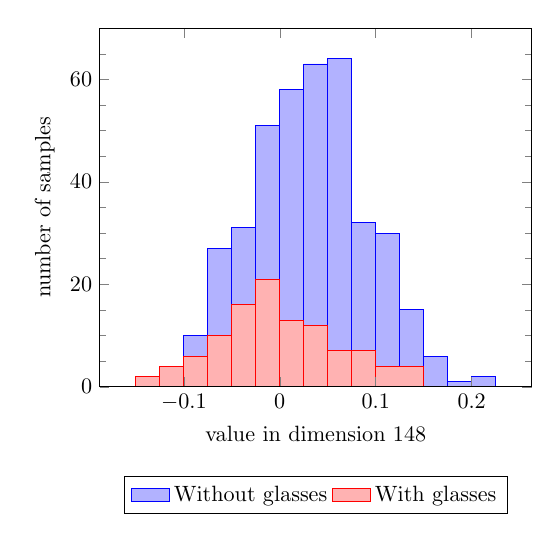
\begin{tikzpicture}[scale=0.8]
        \begin{axis}[
            ymin=0, ymax=70, minor y tick num = 3,
            area style,
            legend style = {
                at = {(0.5, -0.25)},
		        anchor = north,
		        legend columns = -1
		    },
		    ylabel = number of samples,
		    xlabel = value in dimension 148
        ]
            \addplot+[ybar interval, mark=no]
            plot coordinates {
                (-0.150, 2) (-0.125, 2) (-0.100, 10) (-0.075, 27) (-0.050, 31) (-0.025, 51) (0.000, 58) (0.025, 63) (0.050, 64) (0.075, 32) (0.100, 30) (0.125, 15) (0.150, 6) (0.175, 1) (0.200, 2) (0.225, 2) 
            };
            \addplot+[ybar interval, mark=no]
            plot coordinates {
                (-0.150, 2) (-0.125, 4) (-0.100, 6) (-0.075, 10) (-0.050, 16) (-0.025, 21) (0.000, 13) (0.025, 12) (0.050, 7) (0.075, 7) (0.100, 4) (0.150, 2)
            };
            \legend{Without glasses, With glasses}
        \end{axis}
    \end{tikzpicture}
    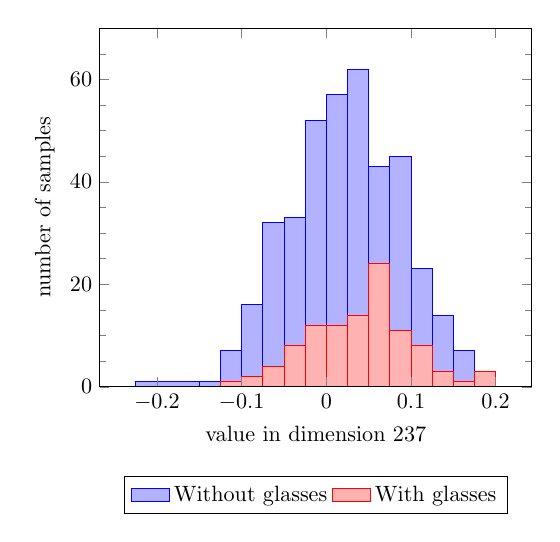
\begin{tikzpicture}[scale=0.8]
        \begin{axis}[
            ymin=0, ymax=70, minor y tick num = 3,
            area style,
            legend style = {
                at = {(0.5, -0.25)},
		        anchor = north,
		        legend columns = -1
		    },
		    ylabel = number of samples,
		    xlabel = value in dimension 237
        ]
            \addplot+[ybar interval, mark=no]
            plot coordinates {
                (-0.225, 1) (-0.150, 1) (-0.125, 7) (-0.100, 16) (-0.075, 32) (-0.050, 33) (-0.025, 52) (0.000, 57) (0.025, 62) (0.050, 43) (0.075, 45) (0.100, 23) (0.125, 14) (0.150, 7) (0.175, 3)
            };
            \addplot+[ybar interval, mark=no]
            plot coordinates {
                (-0.125, 1) (-0.100, 2) (-0.075, 4) (-0.050, 8) (-0.025, 12) (0.000, 12) (0.025, 14) (0.050, 24) (0.075, 11) (0.100, 8) (0.125, 3) (0.150, 1) (0.175, 3) (0.200, 1)
            };
            \legend{Without glasses, With glasses}
        \end{axis}
    \end{tikzpicture}
    \caption{\label{fig:dimension-analysis-histograms}Distribution of samples with values from dimensions number 148 and 237.}
\end{figure}

\subsection*{Results of Student's t-test}
It is clear that some dimensions of a latent space have a larger impact on the feature than the others but no single one of them can be used to determine a feature. Therefore, the proposed hypothesis is rejected. However, a combination of certain dimensions could be used for the latent space analysis. This approach is discussed in the following section.

\section{\label{sec:lda}Linear Discriminant Analysis for latent space projection}
If one single dimension cannot be used to separate the features, a linear combination of multiple dimensions might be better for this task. In this thesis, a technique called Linear Discriminant Analysis (LDA) is discussed. It projects data to a lower-dimensional space where the class-separability is better \cite{duda2001patternclassification}. The hypothesis proposed in this section is as follows. \uv{Latent space can be projected to a subspace in a way that makes the classes of features of a face generated from a point in that latent space separable.}

Input data for this analysis are 256-dimensional vectors representing a single point in a~256-dimensional latent space. The calculation is focusing on data with the feature of glasses presence on a person's face, which means a feature with 2 classes. LDA assumes normally distributed data, statistically independent features (in this case, features are the dimensions of latent space), and identical covariance matrices for every class. The fulfillment of these assumptions is explained in \autoref{sec:analysis-assumptions}.

\subsection*{Calculation of Linear Discriminant Analysis}
The first step of LDA is calculating of 256-dimensional mean vectors $ \pmb m_i$ for each of the classes $i$. This vector contains, as the name suggests, the mean value of the samples in all of their 256 dimensions. $D_i$ is a set of all samples $\pmb x$ in class $i$ and its cardinality is $n_i$.

$$
\pmb m_i =
\begin{bmatrix}
    \mu_{i_{1}}\\
    \mu_{i_{2}}\\
    \vdots\\
    \mu_{i_{255}}\\
    \mu_{i_{256}}\\
\end{bmatrix},
\quad \text{with}\quad i = 0, 1
\quad \quad \quad \quad
\pmb m_i = \frac{1}{n_i} \sum\limits_{\pmb x \in D_i}^{n_i} \; \pmb x
$$

In the next step, $256\times 256$-dimensional within-class and between-class scatter matrices are computed. These matrices are used to make estimates of covariance matrices. The within-class scatter matrix $S_W$ is computed by the following formula, where $c$ is the number of classes. Indexing of classes starts at 0, therefore, $c-1$ is used in the formulas.

$$
S_W = \sum\limits_{i=0}^{c-1}  S_i
,\quad \text{where} \quad
S_i = \sum\limits_{\pmb x \in D_i}^n (\pmb x - \pmb m_i)\;(\pmb x - \pmb m_i)^\top
$$

\noindent And between-class scatter matrix $S_B$ is computed by the following formula, where $\pmb m$ is the overall mean of data and $N_i$ is the cardinality of a sample set of the respective class.

$$
S_B = \sum\limits_{i=0}^{c-1} N_{i} (\pmb m_i - \pmb m) (\pmb m_i - \pmb m)^\top
$$

In the following step, linear discriminants are computed by solving the generalized eigenvalue problem for matrix $S^{-1}_W S_B$. The computed eigenvectors and eigenvalues are important information about the distortion of a linear transformation. Eigenvectors are basically the direction of distortion and their length is 1. Eigenvalues describe the magnitude of this distortion, they scale the eigenvectors. When performing the LDA, eigenvectors are forming the axes of a new subspace and eigenvalues are giving information about how important are respective eigenvectors for the separation of classes.

For LDA, the number of linear discriminants $d$ is at most $c-1$, in other words, one less than the number of classes. That means that for the glasses presence feature, latent space can be only projected to 1-dimensional space when using the LDA ($d=1$). The eigenvalues can be sorted in decreasing order to determine the number of chosen linear discriminants $d$. Respective eigenvectors of chosen eigenvalues are forming the eigenvector matrix $\pmb W$, in this case, it is $256\times 1$-dimensional. Matrix $\pmb W$ is used to transform $n\times 256$-dimensional data $\pmb X$ to $n\times 1$-dimensional data $\pmb Y$.

$$
\pmb Y = \pmb X \times \pmb W
$$

\subsection*{Implementation of Linear Discriminant Analysis}
Python's library \texttt{scikit-learn} already has an implementation of LDA, therefore, it is not necessary to implement it manually \cite{scikit-learn}. The implemented LDA model\footnote{More information about scikit-learn LDA model in library's API at \url{https://scikit-learn.org/stable/modules/generated/sklearn.discriminant_analysis.LinearDiscriminantAnalysis.html}} will perform the operations faster and it is also easier to use. But the main reason for using the \texttt{scikit-learn} LDA model is that it can also serve as a classifier. The model can be saved into a file for later use with the \texttt{joblib} library. Function \texttt{dump} saves it to a file and function \texttt{load} takes care of loading the model when it is used later\footnote{Official website of joblib library with further details at \url{https://joblib.readthedocs.io/en/latest/persistence.html}}.

The main parameter when initializing the model is a number of components, this is the dimensionality of a subspace the data are projected into. Then the model is trained using the \texttt{fit} method provided with the original data (latent points) and their labels (classes). Method \texttt{transform} does the projecting of data into a subspace. In \autoref{fig:lda-transform-glasses} can be seen the transformed samples of latent points labeled with the feature of glasses presence. It~is clear that the classes can be separated and therefore the initial hypothesis, whether the samples can be projected to a subspace where the classes are separable, is accepted for a~feature with 2 classes.

\begin{figure}[!h]
    \centering
    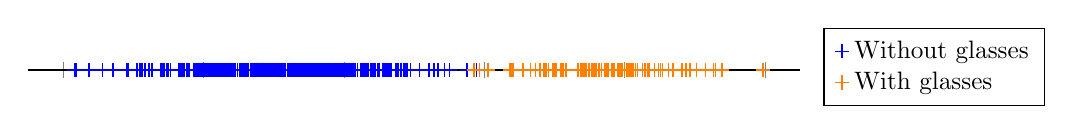
\begin{tikzpicture}[scale=1.3]
        \begin{axis}[
            xmin=-4.5, xmax=6.5,
            ymin=0, ymax=1,
            legend pos = outer north east,
            legend style={nodes={scale=0.7, transform shape}}, 
            legend image post style={mark=+},
            legend cell align={left},
		    axis x line = bottom,
		    x axis line style = -,
		    xticklabels={,,},
            hide y axis,
		    unit vector ratio = {2 1.1}
        ]
            \addplot+[only marks, mark = +, mark options={draw=blue}]
            plot coordinates {
                (-0.657, 0) (-1.963, 0) (-0.239, 0) (-0.680, 0) (-2.105, 0) (0.417, 0) (-2.211, 0) (-0.915, 0) (0.809, 0) (0.401, 0) (-0.983, 0) (0.327, 0) (-2.076, 0) (-0.797, 0) (-1.799, 0) (0.277, 0) (-2.274, 0) (-3.639, 0) (-0.132, 0) (-1.188, 0) (-1.467, 0) (-1.095, 0) (-3.843, 0) (-2.248, 0) (-1.660, 0) (-1.278, 0) (-0.437, 0) (0.303, 0) (-2.735, 0) (-0.849, 0) (-2.894, 0) (-1.197, 0) (0.029, 0) (-1.274, 0) (-1.156, 0) (0.020, 0) (-0.176, 0) (-0.511, 0) (-0.061, 0) (-1.396, 0) (-1.625, 0) (-1.447, 0) (-1.663, 0) (-1.736, 0) (-3.643, 0) (-1.378, 0) (0.074, 0) (0.565, 0) (-1.638, 0) (-0.843, 0) (-0.112, 0) (1.339, 0) (-1.850, 0) (0.110, 0) (-1.709, 0) (-1.864, 0) (-0.037, 0) (-1.655, 0) (-0.491, 0) (-0.895, 0) (-1.734, 0) (-2.345, 0) (-1.917, 0) (0.071, 0) (1.282, 0) (-0.594, 0) (-2.127, 0) (0.670, 0) (-2.772, 0) (-0.698, 0) (-2.228, 0) (-0.044, 0) (-0.899, 0) (-1.008, 0) (-2.298, 0) (-1.864, 0) (-2.095, 0) (-1.400, 0) (-2.882, 0) (-1.165, 0) (-0.731, 0) (0.479, 0) (-0.957, 0) (-0.303, 0) (-1.474, 0) (-0.213, 0) (-1.775, 0) (-0.371, 0) (-0.311, 0) (-2.147, 0) (0.130, 0) (-1.442, 0) (-0.399, 0) (-0.935, 0) (-1.359, 0) (-0.421, 0) (0.848, 0) (-0.499, 0) (-1.642, 0) (-1.995, 0) (-0.088, 0) (-1.366, 0) (-3.094, 0) (-1.171, 0) (0.283, 0) (0.288, 0) (-2.063, 0) (-1.863, 0) (-2.356, 0) (-0.219, 0) (-1.794, 0) (-2.787, 0) (-0.727, 0) (-2.112, 0) (-1.313, 0) (0.584, 0) (-0.923, 0) (-0.787, 0) (-2.846, 0) (-1.636, 0) (-0.851, 0) (-1.906, 0) (-0.875, 0) (-0.220, 0) (0.899, 0) (-1.257, 0) (-1.429, 0) (-1.198, 0) (-0.093, 0) (-0.222, 0) (-0.000, 0) (-0.931, 0) (-0.344, 0) (-1.060, 0) (-2.289, 0) (-1.213, 0) (-0.591, 0) (-0.971, 0) (-1.831, 0) (-0.485, 0) (-1.039, 0) (-0.975, 0) (0.413, 0) (0.094, 0) (-2.022, 0) (0.194, 0) (-1.253, 0) (-1.517, 0) (-0.063, 0) (0.495, 0) (-0.564, 0) (-1.921, 0) (-0.228, 0) (-2.611, 0) (-0.365, 0) (-0.293, 0) (-0.229, 0) (-0.200, 0) (-1.007, 0) (-1.857, 0) (-2.898, 0) (-2.343, 0) (-0.719, 0) (-1.077, 0) (-1.851, 0) (0.375, 0) (-0.726, 0) (-0.704, 0) (0.134, 0) (0.335, 0) (0.656, 0) (-0.650, 0) (-0.834, 0) (-1.068, 0) (-1.771, 0) (-0.868, 0) (0.773, 0) (-0.223, 0) (0.068, 0) (0.130, 0) (-1.316, 0) (-0.647, 0) (-1.417, 0) (-1.224, 0) (0.069, 0) (-1.254, 0) (-0.348, 0) (-0.758, 0) (-1.318, 0) (-0.715, 0) (0.071, 0) (-0.672, 0) (-1.853, 0) (-0.051, 0) (-1.309, 0) (-1.998, 0) (0.546, 0) (-0.555, 0) (-1.560, 0) (-0.730, 0) (-1.015, 0) (-3.071, 0) (-0.428, 0) (-0.575, 0) (-0.279, 0) (0.442, 0) (0.559, 0) (-0.710, 0) (-1.325, 0) (-0.684, 0) (-2.224, 0) (1.430, 0) (0.268, 0) (-0.806, 0) (0.060, 0) (-1.251, 0) (-1.896, 0) (-0.102, 0) (-1.150, 0) (-2.836, 0) (-2.023, 0) (-0.669, 0) (-1.422, 0) (-2.889, 0) (0.135, 0) (-2.363, 0) (-0.457, 0) (-2.139, 0) (-1.298, 0) (-1.596, 0) (0.806, 0) (-0.258, 0) (0.013, 0) (-0.001, 0) (-1.239, 0) (-0.299, 0) (-0.691, 0) (-1.372, 0) (-0.733, 0) (-2.949, 0) (-2.513, 0) (-1.063, 0) (-0.045, 0) (-0.665, 0) (-1.487, 0) (-1.847, 0) (-1.983, 0) (1.753, 0) (-0.357, 0) (-0.473, 0) (-3.293, 0) (0.944, 0) (1.501, 0) (-0.977, 0) (-1.651, 0) (-0.159, 0) (0.442, 0) (0.819, 0) (-2.911, 0) (-1.741, 0) (-1.021, 0) (-0.251, 0) (-1.187, 0) (-1.749, 0) (-1.937, 0) (-1.128, 0) (-0.532, 0) (0.300, 0) (0.597, 0) (-2.314, 0) (-0.610, 0) (-2.074, 0) (-1.691, 0) (0.765, 0) (-0.923, 0) (0.412, 0) (-1.009, 0) (-0.737, 0) (-3.821, 0) (0.238, 0) (-3.443, 0) (-1.450, 0) (0.579, 0) (-0.526, 0) (-1.442, 0) (-2.782, 0) (-1.586, 0) (-1.088, 0) (-0.335, 0) (-2.845, 0) (0.615, 0) (1.208, 0) (-0.379, 0) (-0.799, 0) (-2.298, 0) (-0.880, 0) (-1.142, 0) (-1.078, 0) (-1.485, 0) (-0.687, 0) (-1.233, 0) (-1.916, 0) (-0.574, 0) (-1.813, 0) (0.117, 0) (-0.881, 0) (0.349, 0) (-0.834, 0) (-0.750, 0) (-0.883, 0) (-0.410, 0) (-0.288, 0) (-0.999, 0) (-1.972, 0) (-1.152, 0) (1.888, 0) (-2.747, 0) (-0.576, 0) (-0.605, 0) (-2.474, 0) (-0.624, 0) (-2.569, 0) (-0.471, 0) (-1.945, 0) (-0.801, 0) (-1.149, 0) (-1.763, 0) (-2.020, 0) (-1.189, 0) (-1.743, 0) (-0.419, 0) (-1.108, 0) (-1.218, 0) (0.869, 0) (-2.558, 0) (-2.280, 0) (-2.040, 0) (-0.634, 0) (0.110, 0) (-0.347, 0) (-1.876, 0) (-2.084, 0) (-0.078, 0) (-2.014, 0) (-0.018, 0) (0.390, 0) (-1.147, 0) (-2.004, 0) (0.146, 0) (-0.927, 0) (0.135, 0) (-1.280, 0) (-1.461, 0) (0.046, 0) (-0.319, 0) (-0.856, 0) (-0.447, 0) (-1.363, 0) (-1.557, 0) (-1.161, 0) (-1.457, 0) (-0.853, 0) (-2.039, 0) (-1.138, 0) (-2.785, 0) (-1.577, 0) (-2.582, 0) (-1.780, 0) (-1.369, 0) (0.238, 0) (-1.060, 0) (-2.325, 0) (-1.674, 0) (0.396, 0) (1.077, 0) (-1.836, 0) (0.643, 0) (-1.402, 0) (-0.544, 0) (-2.136, 0) (0.404, 0) (-1.544, 0) (-0.384, 0) (-2.143, 0) (-2.525, 0) (-0.012, 0) (-0.007, 0) (0.164, 0) (0.738, 0) (-0.287, 0) (-1.150, 0) (-2.326, 0) (-0.959, 0) (0.159, 0) (-1.243, 0) (-3.443, 0)
            };
            \addplot+[only marks, mark = +, mark options={draw=orange}]
            plot coordinates {
                (2.785, 0) (3.325, 0) (4.510, 0) (5.290, 0) (3.750, 0) (1.851, 0) (2.841, 0) (4.421, 0) (2.785, 0) (3.161, 0) (4.536, 0) (3.541, 0) (3.532, 0) (3.709, 0) (4.183, 0) (2.793, 0) (2.983, 0) (1.930, 0) (4.031, 0) (3.845, 0) (2.051, 0) (3.084, 0) (3.547, 0) (3.101, 0) (3.939, 0) (4.932, 0) (3.770, 0) (2.546, 0) (3.381, 0) (5.269, 0) (5.386, 0) (4.826, 0) (3.741, 0) (2.730, 0) (2.879, 0) (3.434, 0) (2.410, 0) (3.723, 0) (5.971, 0) (2.361, 0) (4.875, 0) (2.974, 0) (3.728, 0) (3.820, 0) (5.022, 0) (3.668, 0) (4.251, 0) (4.344, 0) (2.543, 0) (3.896, 0) (2.412, 0) (3.407, 0) (2.794, 0) (2.910, 0) (4.811, 0) (4.626, 0) (4.480, 0) (3.131, 0) (3.971, 0) (2.552, 0) (3.374, 0) (3.577, 0) (3.495, 0) (4.073, 0) (2.862, 0) (4.689, 0) (5.155, 0) (3.453, 0) (4.117, 0) (4.293, 0) (4.335, 0) (4.357, 0) (3.103, 0) (4.152, 0) (4.155, 0) (3.931, 0) (3.593, 0) (3.760, 0) (3.380, 0) (3.910, 0) (3.390, 0) (3.998, 0) (3.003, 0) (4.121, 0) (3.589, 0) (3.023, 0) (3.431, 0) (5.265, 0) (4.123, 0) (3.954, 0) (4.332, 0) (4.030, 0) (4.281, 0) (4.059, 0) (3.632, 0) (3.491, 0) (2.379, 0) (2.986, 0) (4.023, 0) (5.149, 0) (3.340, 0) (2.659, 0) (3.855, 0) (4.088, 0)
            };
            \addlegendentry{Without glasses}
            \addlegendentry{With glasses}
        \end{axis}
    \end{tikzpicture}
    \caption{500 samples of faces labeled with glasses presence transformed from \mbox{256-dimensional} space to 1-dimensional space using LDA.}
    \label{fig:lda-transform-glasses}
\end{figure}

LDA model can also be used to transform and classify multi-class samples such as faces labeled with hair color. 4 different classes were chosen for this feature: blond, brown, black, and gray hair. The number of components for the model is set to a maximum value of 3, one lower than the number of classes. \autoref{fig:lda-transform-hair-color} displays the transformed samples. LDA managed to project the samples into such subspace where the classes are separable and therefore the initial hypothesis holds for multi-class samples.

\begin{figure}[!h]
    \centering
    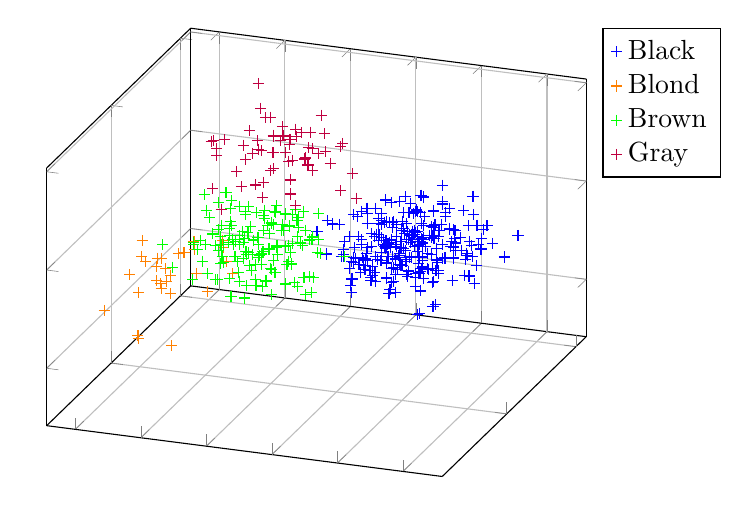
\begin{tikzpicture}[scale=1]
        \begin{axis}[
            grid = major,
            view = {200}{30},
            xticklabels={,,},
            yticklabels={,,},
            zticklabels={,,},
            legend pos = outer north east, 
            legend image post style={mark=+},
            legend cell align={left}
        ]
        	\addplot3+[only marks, mark = +, mark options={draw=blue}] 
        		plot coordinates {
        		    (-1.110, -1.001, -0.982) (-1.982, -0.768, -0.033) (-2.329, 0.300, 0.530) (-2.579, 0.945, -0.854) (-0.406, -0.167, -2.197) (-0.964, -0.196, -2.025) (-0.542, -0.256, 0.942) (-2.418, -0.887, -0.941) (-0.827, 1.464, 0.163) (-0.899, 1.095, -1.553) (-0.865, -0.209, -0.540) (-1.891, -0.983, -0.439) (-1.278, -0.244, 0.715) (-2.515, -0.494, -0.330) (-2.095, 0.429, -0.343) (-2.797, -0.338, 0.423) (-0.157, 0.163, 0.748) (-1.717, -0.210, -1.727) (-1.741, -1.745, -0.587) (-2.437, -0.114, 1.692) (-0.860, 1.083, -0.698) (-1.777, -1.689, -1.263) (-0.775, 0.053, 1.482) (-2.684, 0.249, -2.033) (-3.598, -0.673, 1.648) (-0.467, -0.736, -0.583) (-0.685, 0.410, -0.634) (-1.906, -0.313, -0.432) (-1.237, -0.886, 0.380) (-0.796, -0.967, 0.926) (-3.969, 0.788, 1.665) (-1.772, -0.872, -0.365) (-2.599, -0.007, -1.101) (-2.652, 0.250, -3.186) (-3.631, -0.804, -0.622) (-1.326, 1.197, -0.383) (-1.847, -1.248, -0.996) (-1.397, 0.523, -1.163) (-2.616, -0.708, -0.853) (-0.546, 0.346, 0.335) (-2.093, 0.851, -0.545) (-2.566, -2.501, -1.501) (-0.414, 0.495, -0.502) (-0.524, 0.625, 0.271) (-2.511, -1.160, -0.351) (-0.720, -0.504, 1.243) (-1.546, -1.016, -0.972) (-2.599, 0.454, -1.683) (-1.424, -0.183, 2.028) (-3.856, 0.759, -0.907) (-1.832, -0.538, 0.413) (-3.754, 1.724, -1.503) (-1.518, 0.079, -0.066) (-3.103, 1.510, -2.287) (-0.122, -0.799, -1.778) (-1.526, -1.724, 0.841) (-1.596, 0.292, 0.028) (-3.804, -0.863, 2.268) (-2.295, -0.855, 1.893) (-0.036, -0.405, -0.925) (-0.625, -0.769, 0.789) (-1.317, -1.759, 0.278) (-1.497, -0.801, 0.396) (-1.741, 0.144, -1.867) (-2.281, -2.233, 0.607) (-2.600, 0.078, -1.176) (-1.838, 0.723, -1.231) (-1.727, 0.615, 0.358) (-1.622, -0.008, -2.355) (-3.497, 1.365, -0.645) (-2.256, -0.974, -0.221) (-2.413, -1.938, 1.795) (-1.284, -0.234, 0.905) (-0.322, 1.494, 0.194) (-1.499, 1.508, -0.326) (-2.446, 1.879, -0.901) (-1.777, 0.249, 0.400) (-1.726, 0.563, 0.181) (-3.767, -1.029, -2.282) (-2.874, -1.647, -0.172) (0.302, -0.094, 0.676) (-1.609, -1.752, 0.313) (-2.885, 0.592, -0.187) (-3.345, 0.568, -0.650) (-1.437, 0.979, -0.748) (-1.208, -0.419, 1.132) (-2.141, -0.095, 0.655) (-2.138, -0.957, -0.617) (-3.873, -0.331, -0.352) (-0.812, 0.292, -1.053) (-1.393, -2.410, -1.169) (-1.673, -0.842, 0.561) (-2.171, -0.307, -0.832) (-1.604, 1.201, -0.812) (-3.115, -2.153, -0.255) (-3.130, -0.432, -0.727) (-1.319, 0.064, 0.101) (-4.165, -1.405, -0.433) (-2.237, -0.980, -0.330) (-3.260, -0.739, -0.348) (-1.352, -0.614, -0.455) (-2.597, -1.724, 0.406) (-3.039, 1.162, -0.466) (-2.821, 0.378, -1.287) (-1.636, -0.793, -0.743) (-2.021, -1.032, 1.085) (-2.279, 0.728, -0.486) (-1.949, -0.660, 0.035) (-0.551, -0.853, -1.346) (-1.416, -2.254, -1.131) (-3.811, -1.581, 0.069) (-3.723, -1.651, -0.438) (-1.852, -1.683, 0.462) (-2.975, -2.887, -0.247) (-1.485, -0.200, -0.250) (-0.784, -0.113, -1.133) (-2.714, 0.201, -0.329) (-2.900, -0.751, 0.725) (-0.644, -0.347, -1.174) (-1.570, 0.886, -1.341) (-3.087, -0.918, -0.482) (-1.954, 0.361, -2.195) (-1.095, 0.525, -1.084) (-1.906, 0.442, -0.331) (-2.080, -1.043, -0.527) (-0.114, -0.108, -1.072) (-1.303, -0.902, 1.388) (-1.665, 1.178, 1.175) (-2.354, -0.278, -0.448) (-2.601, -0.066, -0.545) (-2.895, -0.237, 0.462) (-3.059, 0.048, -1.030) (-3.243, 0.349, -0.401) (0.368, 0.531, 0.541) (-3.217, 0.666, -0.501) (-1.675, -0.657, -0.333) (-2.477, -0.047, -0.885) (-1.901, 0.701, -2.019) (-2.350, 0.797, -0.422) (-1.529, -1.462, -0.020) (-2.703, 0.406, -0.213) (-1.933, 0.231, 0.063) (-2.676, -0.704, 1.383) (-2.122, -0.598, 0.352) (-1.629, 0.630, -0.060) (-1.618, -0.415, -1.090) (-2.447, -1.561, -0.541) (-3.505, 0.128, 1.185) (-2.191, -2.996, -0.168) (-1.994, -1.388, 1.578) (-2.839, -0.671, -1.746) (-2.565, -1.623, -0.967) (-2.093, 0.566, -0.832) (-1.014, 0.631, -1.183) (-3.146, -2.174, -1.079) (-2.403, -1.331, 0.040) (-1.611, -1.945, 0.345) (-3.431, -0.042, 1.128) (-0.739, -0.804, -0.916) (-2.832, -0.302, -1.904) (-0.515, -0.998, 0.080) (-1.035, -1.044, -1.009) (-2.553, -0.964, -0.231) (-1.243, -1.404, -0.723) (-3.262, -0.814, 0.049) (0.005, -1.389, -2.064) (-1.339, -0.954, 0.382) (-2.238, 1.037, 0.793) (-1.565, -2.680, -0.509) (-1.679, 0.442, 0.065) (-3.240, -1.586, -2.360) (-0.672, -1.482, -0.764) (-2.265, -0.770, -0.163) (-1.231, -0.811, -0.667) (-1.659, 1.706, 0.313) (-2.830, -0.162, 0.975) (-1.927, -1.166, -2.476) (-2.934, -0.253, -0.158) (-1.139, -1.877, 0.749) (-4.610, -2.206, -0.477) (-5.198, 0.168, 0.179) (-1.745, -2.074, -1.381) (-1.332, 2.065, -1.153) (-0.734, -1.103, -1.640) (-2.402, 0.762, 1.178) (-1.926, 0.466, -1.580) (-1.487, -0.488, -1.631) (-3.284, -1.190, -0.179) (-4.111, 0.150, -1.033) (-1.332, 0.158, -0.775) (-2.131, -0.231, -0.754) (-3.546, 0.065, 0.531) (-2.365, -1.025, -1.873) (-0.857, -1.011, 0.390) (-3.714, -1.298, -1.561) (-2.156, -0.250, -0.035) (-2.526, -1.139, 0.340) (-3.248, 0.276, 1.192) (-1.849, -0.603, 2.002) (-2.289, -0.323, 1.556) (-2.034, -1.460, -0.014) (-1.376, 0.722, 0.251) (-3.438, -0.340, -0.598) (-0.777, -0.003, -0.257) (-1.481, -0.433, -0.559) (-3.064, 1.296, -0.275) (-1.679, -0.099, 0.984) (-1.911, -0.722, 1.109) (-1.953, 2.125, -0.366) (-1.711, 0.803, 0.861) (-0.799, -0.981, -0.384) (-1.726, -0.598, -0.317) (-2.512, 2.220, 1.010) (-2.136, -0.412, 0.229) (-2.353, 0.049, 0.804) (-1.437, -1.604, -1.504) (-3.536, -0.638, -0.380) (-2.644, -0.977, -1.305) (-2.996, -0.756, 1.327) (-1.920, 1.262, 0.252) (-2.659, 0.577, -0.912) (-4.247, -0.826, 0.889) (-2.067, 0.308, -0.795) (-2.299, -0.730, 0.664) (-2.003, 2.636, 1.082) (-2.474, -0.029, 0.487) (-2.564, -1.606, 1.221) (-0.922, -1.303, 0.011) (-3.635, -0.739, -0.893) (-2.771, -1.945, -0.443) (-1.067, 1.261, -0.258) (-1.310, -3.162, 0.128) (0.089, -1.782, -1.235) (0.044, -1.441, -1.566) (-0.280, 0.970, 1.352) (-2.932, 0.995, 0.271) (-1.449, 0.421, 1.251) (-4.156, 0.048, 0.440) (-1.322, -0.145, -1.042) (-2.687, 1.372, 0.325) (-2.517, -0.779, 0.057) (-2.350, -0.682, -0.488) (-1.884, -0.256, 0.544) (-2.772, -2.023, -1.501) (-1.247, -0.670, 0.577) (-3.515, 0.666, 0.074) (-2.793, 0.061, -1.004) (-0.193, -0.785, 0.594) (-1.118, -1.323, -0.851) (-2.235, -0.949, -0.342) (-3.774, -0.906, -0.856) (-1.619, 0.234, -0.850) (-2.536, 0.815, -0.665) (-0.958, -1.315, -0.915) (-2.660, 1.243, -0.514) (-0.688, -0.975, -2.076) (-1.579, -0.786, -1.179) (-4.157, -0.603, -0.168) (-1.604, -0.232, 0.654) (-1.407, 0.776, 0.998) (-4.130, -0.477, 0.130) (-2.024, 1.604, 0.299) (-1.974, 1.253, 1.054) (-1.391, -1.367, -1.259) (-2.109, 0.437, -0.138) (-3.640, -1.537, 0.302) (-2.869, -0.185, -3.071) (-2.632, 0.044, -0.968) (-1.805, -0.752, -1.386) (-2.771, -0.315, 0.317)
        		};
        		\addplot3+[only marks, mark = +, mark options={draw=orange}] 
        		plot coordinates {
        		    (5.118, -0.230, -6.827) (5.762, -0.938, -4.291) (5.890, -1.618, -4.011) (6.093, -1.491, -3.437) (5.651, 0.960, -5.602) (5.151, -0.218, -4.181) (3.577, -0.972, -3.335) (4.989, -1.536, -2.791) (4.086, -1.534, -2.484) (4.289, -0.819, -4.302) (5.829, -0.803, -4.065) (4.668, -0.758, -1.795) (5.171, -0.225, -3.233) (6.725, 0.851, -4.630) (4.682, -2.842, -3.176) (6.186, -0.586, -2.738) (6.308, -0.901, -2.177) (5.185, -0.862, -2.586) (6.095, -1.459, -3.827) (4.403, -0.298, -3.035) (5.633, -0.667, -4.322) (5.932, -1.403, -3.349) (5.834, 0.503, -6.109) (3.860, -1.203, -2.914) (5.951, 0.183, -4.012) (5.088, -1.036, -2.614) (5.276, -0.231, -3.568) (6.874, -1.333, -4.343) (5.862, -0.116, -2.629)
        		};
        		\addplot3+[only marks, mark = +, mark options={draw=green}] 
        		plot coordinates {
        		    (0.400, 2.217, 2.525) (2.158, -0.403, -0.011) (1.151, 2.807, 0.685) (1.001, 1.334, 1.835) (0.626, 2.173, 0.845) (1.481, 1.070, 1.029) (-0.282, 1.814, 0.444) (0.810, 0.472, 1.429) (1.230, 2.443, 0.640) (2.845, 0.865, 1.796) (1.182, 1.089, 1.112) (3.780, 2.917, -0.377) (2.893, 3.483, 1.431) (3.049, 3.092, 1.051) (1.971, 1.962, 0.808) (0.992, 2.912, 2.058) (0.803, -0.138, -0.425) (2.016, 2.246, 0.668) (1.038, 3.352, -0.409) (1.986, 3.814, 1.478) (3.344, 1.261, 1.092) (2.293, 2.938, 0.159) (1.047, 3.996, -0.003) (2.003, 3.404, 1.479) (0.489, 1.868, -1.183) (1.477, 3.125, -1.318) (2.853, 1.648, 0.514) (3.088, 2.240, 2.981) (2.453, 0.896, -0.214) (0.239, 2.045, 1.010) (1.120, 0.814, -0.137) (0.969, 1.277, -0.770) (2.183, 1.201, 1.890) (1.738, 1.093, 1.706) (2.081, 2.807, 1.529) (0.701, 1.070, 1.522) (2.361, 2.179, 0.687) (1.566, 2.824, 0.820) (1.949, 3.535, 0.653) (2.975, 0.682, -2.317) (2.457, 2.759, -0.850) (2.353, -0.905, -0.457) (0.162, 2.776, 1.483) (1.597, 2.721, 0.608) (2.340, 2.074, -2.143) (1.229, 1.343, -0.269) (2.012, 2.045, 1.216) (0.371, 1.467, -1.178) (3.137, 0.548, 1.922) (1.828, 2.224, 2.391) (2.455, 1.596, 0.170) (1.394, 3.715, -0.033) (1.179, 0.006, -0.275) (1.001, 3.485, -0.043) (0.980, 1.118, -0.703) (-0.163, 2.620, -1.142) (2.631, 1.099, -0.849) (1.316, 2.503, 1.016) (1.435, 1.015, 1.597) (3.146, 2.572, 0.410) (0.891, 2.194, 0.769) (1.529, 2.561, 1.932) (0.970, 2.449, -0.172) (-0.215, 2.292, -1.250) (0.659, 3.527, -0.002) (2.351, 1.964, 0.679) (1.206, 2.138, 1.736) (0.776, 1.007, 1.327) (1.186, 2.466, 0.664) (0.028, 3.600, 0.033) (0.955, 2.174, -0.540) (1.768, 2.106, -0.435) (0.512, 2.615, 1.987) (0.549, -0.024, 1.014) (1.283, 1.778, 1.103) (1.295, 2.542, 0.378) (1.086, 0.399, 1.399) (0.198, 0.924, -0.227) (2.896, 2.426, -0.850) (2.615, 2.560, -1.025) (0.264, 1.116, 0.676) (2.725, 1.858, 1.256) (2.018, 2.791, 2.033) (-0.459, 3.045, 0.149) (1.096, 2.715, -0.933) (1.079, 1.744, 2.512) (0.061, 1.825, 1.052) (2.056, 1.698, 1.820) (0.816, 2.725, 0.005) (1.783, 1.857, -0.042) (2.535, 2.702, 0.820) (3.134, 1.546, 0.508) (2.388, 2.030, 1.646) (0.940, 2.065, 0.749) (1.532, 2.485, -0.373) (2.345, 2.077, 2.323) (1.938, 0.636, 0.942) (2.013, 3.496, 0.957) (-0.351, 0.240, -0.788) (3.270, 0.804, 1.585) (0.879, 1.297, 1.234) (0.458, 2.140, -0.042) (1.751, 1.129, 1.468) (0.451, 1.143, 0.998) (1.115, 1.898, -0.148) (2.124, 2.264, 0.851) (1.804, 1.405, 0.537) (2.315, 1.543, 2.068) (1.276, 1.416, 1.969) (1.978, 2.019, -0.169) (1.092, 2.826, 0.803) (0.241, 1.905, 0.781) (0.862, 3.959, 2.335) (1.979, 1.705, 0.947) (4.280, 2.434, 0.313) (2.768, 3.236, 1.422) (1.652, 1.694, 0.749) (2.561, 2.276, 0.571) (3.033, 2.246, 0.464) (2.703, 3.248, 0.375) (1.046, 2.916, 0.339) (2.438, 1.930, 1.204) (0.642, 3.140, -0.971) (-0.003, 1.667, -0.956) (1.612, 2.550, 0.568) (2.419, 4.658, 0.491) (1.499, 3.551, 0.277) (1.191, 0.476, -0.766) (0.930, 1.794, 1.305) (0.650, 3.330, 1.494) (2.722, 2.055, 1.164) (-0.005, 2.831, -0.597) (1.985, 1.090, 1.521) (2.015, 2.262, 1.155) (2.542, 0.970, -0.044) (0.510, 1.543, 1.392) (1.667, 1.869, -0.498) (1.648, 3.260, 0.596) (0.141, 0.987, 0.506) (2.507, 3.475, 3.170) (1.226, 0.472, 0.560)
        		};
        		\addplot3+[only marks, mark = +, mark options={draw=purple}] 
        		plot coordinates {
        		    (3.407, -1.971, 2.142) (1.743, -1.828, 2.314) (4.393, -4.088, 1.635) (4.888, -2.523, 2.044) (5.054, -3.092, 1.681) (1.890, -4.772, 0.911) (1.243, -3.403, 2.137) (1.587, -2.988, 1.926) (1.790, -2.529, 1.230) (3.926, -3.468, -0.598) (2.977, -3.140, 2.811) (2.473, -2.538, -0.109) (0.876, -1.614, 2.417) (2.639, -2.592, 1.909) (0.271, -2.080, 0.460) (2.054, -1.658, 2.303) (4.009, -1.179, -0.294) (3.302, -3.787, 1.600) (4.398, -3.683, 1.182) (2.668, -2.868, 1.288) (2.498, -3.857, 0.456) (2.876, -2.947, 2.477) (3.118, -2.852, 2.452) (4.035, -2.347, 0.835) (2.047, -2.821, 2.133) (2.985, -2.551, 1.056) (4.508, -2.566, 2.191) (2.073, 0.374, 2.566) (4.117, -4.092, 4.098) (4.789, -2.687, 1.598) (2.515, -3.706, 0.914) (2.558, -2.732, 2.514) (1.646, -0.942, 0.551) (3.728, -3.689, 2.709) (3.483, -3.509, 0.203) (3.063, -2.667, 1.794) (4.058, -3.915, 1.309) (3.725, -1.950, 0.395) (2.892, -5.742, 1.618) (2.062, -3.574, 1.329) (2.991, -4.532, 1.546) (2.851, -3.374, 1.770) (2.802, -3.707, 2.323) (0.689, -1.952, 0.846) (2.241, -1.957, 1.051) (1.689, -2.244, 2.580) (3.577, -2.824, 1.738) (2.413, -2.818, 2.629) (2.294, -3.562, 2.373) (2.021, -3.931, 2.099) (4.517, -1.752, 0.252) (3.464, -2.891, -0.722) (0.688, -2.758, 1.158) (3.615, -3.980, 1.656) (3.952, -2.774, 1.155) (4.057, -4.138, 2.826) (2.604, -2.781, 2.474) (3.200, -2.168, 2.188) (4.651, -2.366, 1.481) (3.702, -4.008, 2.535)
        		};
        	\addlegendentry{Black}
            \addlegendentry{Blond}
            \addlegendentry{Brown}
            \addlegendentry{Gray}
    	\end{axis}
    \end{tikzpicture}
    \caption{500 samples of faces labeled with hair color projected from 256-dimensional space to 3-dimensional space using LDA.}
    \label{fig:lda-transform-hair-color}
\end{figure}

\section{\label{sec:generating-features}Generating faces with specific features}
The simplest approach to generating faces with specific features is to generate a large number of latent points (for example 1000) and use the classifier to determine whether the generated face will have the asked features. The first latent point that meets these requirements is used to generate a face. If 1000 generated latent points are not enough, 1000 more are generated and the classifying continues. The latent point has to satisfy all of the conditions for requested features, only then it is accepted.

Classification of features from the latent point can be done by multiple methods of the LDA model, for example, \texttt{predict}, \texttt{predict\_proba}, or \texttt{decision\_function}. LDA classifier for glasses presence was tested on 100 unseen images that were manually labeled and its success rate was 75 \% when using the \texttt{predict} method. To ensure that generated latent point belongs to a face with requested features, a classifying method that offers more information than just hard decisions might be used.

Method \texttt{predict\_proba} gives information about the probability of the sample belonging to each of the classes. The latent point can be then accepted for generating a requested face only in the case where the probability of requested features is multiple times bigger than the probability of other classes of those features. In this thesis the multiplier for latent point acceptance is $10^8$. For example, the probability of a face with glasses has to be $10^8$ higher than the probability of face without glasses, only then is the latent point accepted. This increases the probability of generating the requested face.

An experiment was done to test how the multiplier affects the probability of the requested feature being part of the face. The glasses presence was chosen as a requested feature. For each of the multipliers, 100 images were generated and manually labeled. Results are only approximate but as can be seen in \autoref{tab:multiplier-analysis} higher multiplier can positively affect the generator success rate. In the original dataset of 500 labeled faces, 21 \% of them were with glasses.

\begin{table}[!h]
    \begin{center}
        \begin{tabular}{|l||r|r|r|r|r|}
            \hline
            Multiplier & $1$ & $100$ & $10^4$ & $10^6$ & $10^8$ \\
            \hline
            Probability & 45 \% & 53 \% & 62 \% & 71 \% & 84 \% \\ 
            \hline
        \end{tabular}
    \end{center}
    \caption{\label{tab:multiplier-analysis}Comparison of how the multiplier affects the probability of generating face in the requested class. The multiplier is used to make the difference between the requested class and other classes bigger by multiplying the probability of other classes before comparing with the requested class probability.}
\end{table}

The main hypothesis of this chapter is as follows. \uv{It is possible to generate images with specific characteristics.} Face with requested features can be generated with probability approximately 80 \% and therefore the hypothesis is credible. Generated images of faces with various features can be seen in \autoref{fig:appendix-ffhq-forced}.

Further improvement could be achieved by using the LDA only for projecting of the samples to a subspace and then using another model, such as Support Vector Machine, for classification. Another way of improving the latent space analysis would be to use Quadratic Discriminant Analysis (QDA) instead of Linear Discriminant Analysis. Classes are not always easily linearly separable and by introducing a non-linearity to the process, results could improve.

\chapter{Conclusion}
This thesis had two main goals. The first goal was to design and develop a Generative Adversarial Network (GAN) that is able to generate credible images of faces. And the second goal was to develop a tool that provides an option to generate faces with specific features without any changes to the GAN itself. Both of these goals were completed.

In order to obtain the knowledge necessary to understand how GANs work, different fields of Machine Learning had to be studied. Basic knowledge about Neural Networks and especially Convolutional ones is fundamental to complete this task. Generative Adversarial Networks were then thoroughly studied. Available image databases were reviewed and three were chosen for the implementation.

Three models of GANs were successfully implemented. The first one can generate images of handwritten digits in grayscale. The second one was gradually implemented as~a~variation of the previous GAN and it is able to generate low-resolution color images of faces. Last GAN was focused on higher resolution color images with a large variance in the look of faces and backgrounds and it is capable of generating $128 \times 128$-pixel color images with real-looking faces. 

Latent space that represents a source for generator inputs was analyzed with two methods. A small dataset of faces labeled with information about glasses and hair color was used for the analysis. At first, Student's t-test was used to determine that no single dimension of latent space can be used to separate classes of a feature. Next, Linear Discriminant Analysis was computed to project the latent space to a subspace where the classes of features were separable. This accomplishment leads to the possibility of providing the generator with specific input to generate face with requested features with probability approximately 80 \%. A simple tool that allows a user to set features and generate a face with them is implemented.

The quality of generated images could be improved by using advanced techniques in~GAN design as progressive growing or minibatch standard deviation. As it is very common for Neural Networks, better results could be also achieved with more computational power and longer training process.

Latent space analysis could be improved by an automatic feature recognition to expand the number of possible requested features and to achieve higher precision in the latent space analysis. A non-linear method as Quadratic Discriminant Analysis could be used for the projection into a subspace and an advanced classifier, such as Support Vector Machine, could be used after this projection.
